\documentclass{article}
\usepackage{graphicx} % Required for inserting images
\usepackage[margin=2cm, top=3cm]{geometry} % margine superiore ridotto a 1 cm
\usepackage{listings}
\usepackage{subcaption}  % Pacchetto per sottodidascalie
\usepackage{float}       % Pacchetto per posizionamento rigido delle figure
\usepackage{xcolor} % Pacchetto per i colori
\usepackage{amsmath} % Pacchetto per simboli avanzati

\title{Esame Reti di Calcolatori}
\author{Mattia Cosimi}
\date{December 2024}

\begin{document}

\maketitle

\section{Il modello ISO-OSI}
\subsection{Gli strati del modello ISO-OSI}
\begin{figure}[H]
    \centering
    \begin{minipage}{0.4\textwidth} % Imposta la larghezza della colonna sinistra
        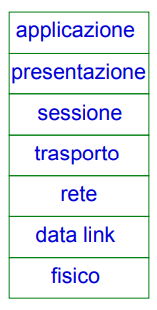
\includegraphics[width=4cm, height=5cm]{Screenshot 2024-12-26 141657.png}
        \label{fig:immagine}
    \end{minipage}%
    \hfill
    \begin{minipage}{0.45\textwidth} % Imposta la larghezza della colonna destra
       Uno strato fornisce a quello immediatamente superiore dei servizi. I servizi sono mostrati in modo via via più astratto man mano che si passa da uno strato ad uno superiore

    \end{minipage}
\end{figure}
\begin{figure}[H]
    \centering
    \begin{minipage}{0.4\textwidth} % Imposta la larghezza della colonna sinistra
        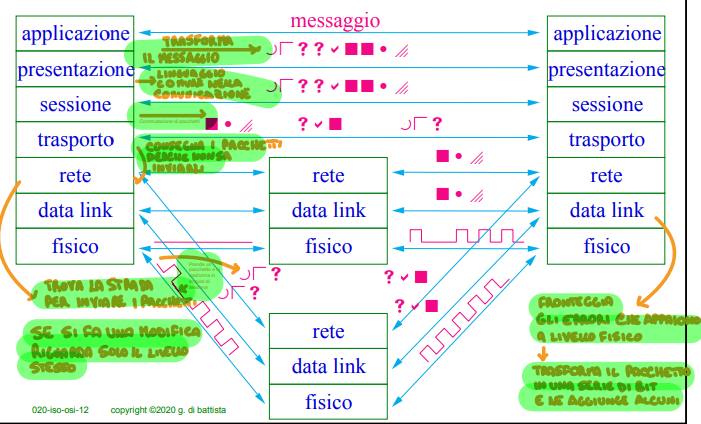
\includegraphics[width=11cm, height=6cm]{Screenshot 2024-12-26 142409.png}
        \label{fig:immagine}
    \end{minipage}%
    \hfill
    \begin{minipage}{0.35\textwidth} % Imposta la larghezza della colonna destra
       In quest'immagine, il livello \textbf{applicazione} trasforma il messaggio ed è il mezzo per accedere alla rete per un processo applicativo, il livello \textbf{presentazione} fa avvenire uno scambio di messaggi utilizzando un linguaggio comune nella comunicazione, nel livello \textbf{sessione} sincronizzazione del dialogo tra due processi, il livello \textbf{trasporto}, colma deficienze e fluttuazioni della qualità del servizio dello strato di \textbf{rete}, consegna i pacchetti al livello di \textbf{rete} il quale trova la strada per inviare i pacchetti, infatti già conosce la topologia (la mappa) della rete. Il livello \textbf{data link} fronteggia gli errori che appaiono a livello fisico e trasforma il pacchetto in una serie di bit. Lo strato \textbf{fisico} si interfaccia direttamente con il mezzo trasmissivo. Offre allo strato superiore una comunicazione indipendentemente dal mezzo trasmissivo. Trasmette e consegna bit.

    \end{minipage}
\end{figure}
\noindent
Il punto logico in cui uno strato offre il servizio allo strato superiore è detto \textbf{Service Access Point (SAP)}. Ogni strato è definito in modo del tutto indipendente dallo strato inferiore. I dati generati da un protocollo di livello n sono detti \textbf{n-pdu (Protocol Data Unit)}, $pdu=header+payload$. Con PDU intendiamo un pacchetto.
\\
\subsection{Servizi e protocolli connessi e non}
Per tutti i livelli superiori al primo sono pensabili due modalità operative, tipi di servizi e di protocolli: connessi o non connessi. Se un servizio è \textbf{connesso} sono disponibili primitive per presentarsi all'interlocutore (instaurare la connessione), per scambiarsi messaggi, per salutare l'interlocutore a trasmissione conclusa (abbattere la connessione) Es. telefonata. Se un servizio è \textbf{non connesso} sono disponibili solo primitive per l'invio di messaggi Es. Mail.
\section{Il progetto IEEE 802}
L'obiettivo è quello di definire un insieme di standard di livello fisico (livello 1) e di livello data-link (livello 2) per far comunicare computer sulla stessa rete locale (LAN), rete personale (PAN) o rete metropolitana (MAN). Da ricordare \textbf{802.3 Ethernet e 802.11 wireless LAN}. IEEE 803 distingue, nel livello 2, i sottolivelli \textbf{MAC e LLC}. I due sottolivelli corrispondono a due tipologie di pacchetti.
\subsection{MAC (Media Access Control)}
Il MAC è specifico per ogni tipo di LAN, infatti i computer che vogliono comunicare devono essere posizionati nella stessa LAN. Ciò richiede la determinazione di due problemi: il primo, \textbf{in ricezione}, la determinazione del destinatario. A tal proposito si utilizzano gli indirizzi \textbf{MAC} (presenti nella MAC pdu) che consentano trasmissioni. Il secondo in trasmissione, se la LAN è realizzata con un unico canale trasmissivo condiviso, va verificata la disponibilità del canale e soluzione di eventuali conflitti.
\subsubsection{MAC pdu e indirizzi MAC}
I seguenti campi sono presenti in ogni tipo di tecnologia prevista dallo standard IEEE 802
\begin{figure}[H] % Usa 'H' per forzare la posizione qui
    \centering % Centra l'immagine
    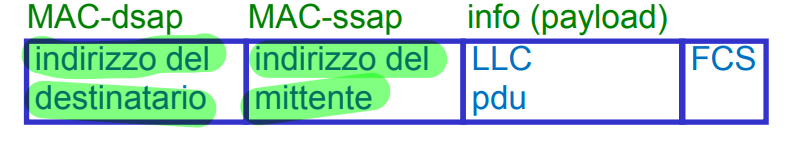
\includegraphics[width=10cm, height=2cm]{Screenshot 2024-12-26 145755.png} % Percorso dell'immagine
    \caption{} % Didascalia per l'immagine
    \label{fig:immagine} % Etichetta per riferimento
\end{figure}
FCS (Frame Check Sequence) serve all'identificazione di eventuali errori.\\\\
Gli \textbf{indirizzi MAC} sono indirizzi di 6 byte rappresentati in notazione esadecimale. Ogni gruppo è di 4 bit, i byte sono separati tra loro da due punti o trattini. Ci sono tre tipi di indirizzi: \textbf{unicast} identificano le singole schede di rete dei computer, se l'ultimo bit del primo byte ha valore 0 allora l'indirizzo è unicast. \textbf{Multicast} identificano gruppi di schede di rete, se l'ultimo bit del primo byte ha valore uno, allora, l'indirizzo MAC è multicast. \textbf{Broadcast} tutte le schede di rete (Tutte FF). Gli indirizzi forniti alle schede di rete sono unici a livello mondiale. I primi 3 byte sono assegnati al costruttore (Organization Unique Identifier), i secondi 3 byte sono definiti dal costruttore. Es. sulle slide. Gli indirizzi MAC possono essere assegnati anche in contesti virtuai e quindi essere amministrati localmente. Se il penultimo bit del primo byte ha valore zero, allora l'indirizzo MAC è unico a livello mondiale e l'unicita è gestita attraverso gli OUI.
\subsection{Il sottolivello LLC}
\begin{figure}[H] % Usa 'H' per forzare la posizione qui
    \centering % Centra l'immagine
    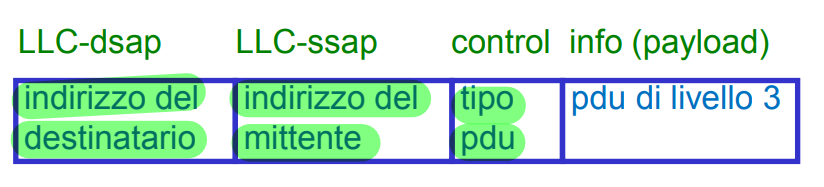
\includegraphics[width=10cm, height=2cm]{Screenshot 2024-12-26 152112.png} % Percorso dell'immagine
    \caption{} % Didascalia per l'immagine
    \label{fig:immagine} % Etichetta per riferimento
\end{figure}
\noindent
LLC-dsap e LLC-ssap servono a denotare i protocolli di livello 3 a cui sono destinati i pacchetti. Consentono la convivenza di diversi protocolli di livello 3 sulla stessa LAN e sulla stessa macchina.
\section{IEEE 802.3 (Ethernet)}
Solitamente per la trasmissione si utilizzano cavi in rame twisted pair o fibre ottiche. La trasmissione è punto-punto bidirezionale tra due stazioni le quali possono trasmettere (e ricevere) contemporaneamente. I pacchetti più piccoli per Ethernet sono da 512 b/s. I più grandi 1500 byte.
\begin{figure}[H] % Usa 'H' per forzare la posizione qui
    \centering % Centra l'immagine
    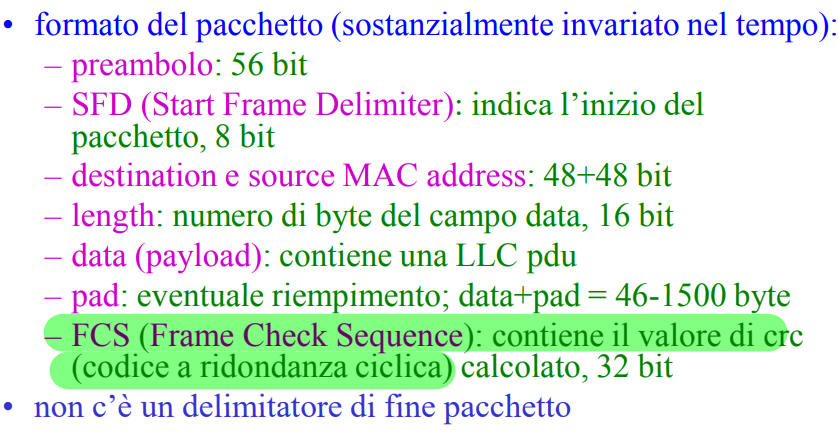
\includegraphics[width=11cm, height=6cm]{Screenshot 2024-12-26 154815.png} % Percorso dell'immagine
    \caption{} % Didascalia per l'immagine
    \label{fig:immagine} % Etichetta per riferimento
\end{figure}
\noindent
Per quanto riguarda le funzioni svolte dal livello MAC, nella \textbf{trasmissione dei pacchetti}: il MAC riceve un pacchetto da LLC, lo incapsula nel pacchetto di livello MAC e lo trasforma in una stringa di bit che viene consegnata al livello fisico per la trasmissione sul mezzo fisico. Nella \textbf{ricezione dei pacchetti} il MAC riceve una stringa di bit dal livello fisico e la interpreta come pacchetto di livello MAC; se il pacchetto è indirizzato ad altri o contiene errori viene scartato, altrimenti la parte MAC viene rimossa e il pacchetto è fornito a LLC. \textbf{Generazione di FCS in trasmissione}: contiene un codice a ridondanza ciclica (CRC) per il controllo degli errori. \textbf{Controlllo di FCS in ricezione}: il MAC verifica che l'FCS ricevuto sia uguale a quello calcolato localmente, i pacchetti ricevuti con errori vengono scartati senza richiesta di ritrasmissione.
\subsection{Reti Ethernet poco comuni}
In passato la comunicazione non era punto-punto bidirezionale, infatti il mezzo trasmissivo era condiviso. Il mezzo trasmissivo si chiamava dominio di collisione dato che i pacchetti potevano collidere. Il mezzo trasmissivo poteva essere realizzato tramite un \textbf{repeater}. In un dominio di collisione un pacchetto spedito da un computer può essere ascoltato da ogni altro computer. \\
Nelle reti locali convivono comunemente pacchetti IEEE 802.3 e pacchetti Ethernet vecchia versione la differenza sta nel fatto che: in Ethernet II (vecchia versione) non c'è lo strato LLC, per cui il pacchetto di livello 3 entra direttamente nel pacchetto di livello MAC. Le funzioni di multiplexing per i protocolli di livello 3 svolti da LLC sono svolti dal campo type, che sostituisce il campo lunghezza di IEEE 802.3.
\subsubsection{Repeater (HUB)}
Il Repeater è situato a livello fisico, ripete il segnale ricevuto da una porta a tutte le altre porte. Non è una macchina store \& forward (non memorizza completamente il pacchetto prima di ritrasmetterlo).
\section{Bridge - Switch}
I bridge, servono a realizzare topologie di reti articolate e con molti computer (switch e bridge sono sinonimi). Vari computer possono essere collegati a un bridge, in modo da formare una rete locale. Le schede del bridge alle quali sono collegati i fili si chiamano porte. I bridge possono anche essere collegati fra loro, consentendo di realizzare reti locali con topologie articolate.
\subsection{funzione di Filtering}
Un bridge cerca di ritrasmettere solo i pacchetti che devono effettivamente transitare da una parte della LAN a un'altra parte della LAN: funzione di filtering. (dagli appunti: separare tra loro porzioni di rete che non devono comunicare in modo diretto.
\begin{figure}[H] % Usa 'H' per forzare la posizione qui
    \centering % Centra l'immagine
    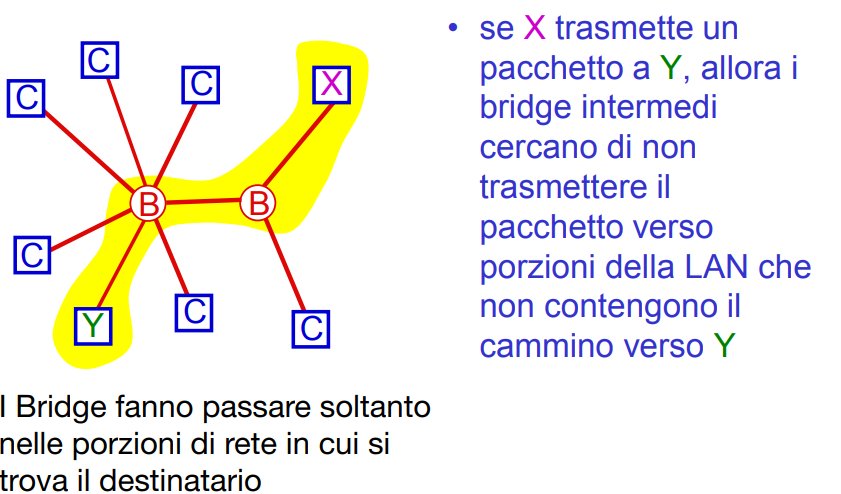
\includegraphics[width=11cm, height=6cm]{immagine_2024-12-26_161613650.png} % Percorso dell'immagine
    \caption{} % Didascalia per l'immagine
    \label{fig:immagine} % Etichetta per riferimento
\end{figure}
\noindent
\subsection{Caratteristiche generali dei bridge}
I bridge ritrasmettono i pacchetti ricevuti con modalità store \& forward (memorizza e ritrasmetti). Ogni pacchetto viene prima ricevuto completamente dal bridge sulla porta di ricezione, poi viene messo in coda (chiamata anche buffer) sulla porta o sulle porte sulle quali deve essere ritrasmesso e poi viene ritrasmesso. Appartengono al livello 2 e utilizzano algoritmi di instradamento semplici per svolgere la funzione di filtering. Devono essere conformi allo standard IEEE 802.1D.
\\
Le porte di un bridge possono avere lo \textbf{stesso MAC} o avere \textbf{MAC differenti}. Nel caso in cui un pacchetto sia ricevuto da una porta con un MAC e ritrasmesso da una porta con un altro MAC occorre effettuare una trauzione di formato del pacchetto, compreso il ricalcolo dell' \textbf{FCS}. Se l'interconnessione è con parti di LAN non conformi a IEEE 802, allora occorre preoccuparsi anche di \textbf{LLC}.
\vspace{150pt}
\subsection{Learning}
I bridge costruiscono la propria tabella di instradamento (detta anche \textbf{filtering database}) con un processo di \textbf{learning}.
\begin{figure}[H] % Usa 'H' per forzare la posizione qui
    \centering % Centra l'immagine
    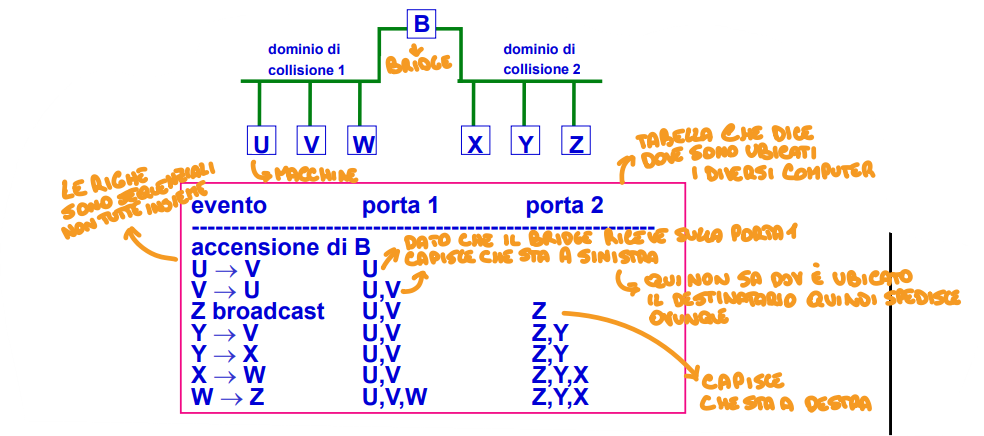
\includegraphics[width=13cm, height=6cm]{Screenshot 2024-12-26 162902.png} % Percorso dell'immagine
    \caption{} % Didascalia per l'immagine
    \label{fig:immagine} % Etichetta per riferimento
\end{figure}
\noindent
La tabella contiene entry (righe) \textbf{statiche} ed entry \textbf{dinamiche}. Il processo di learning si basa sugli indirizzi mittente dei pacchetti ascoltati.
\subsection{Spanning Tree}
Il processo di learning funziona solo se la topologia della LAN è ad \textbf{albero}. La topologia è normalmente a \textbf{grafo (contiene uno o più cicli)}, infatti viene \textbf{dinamicamente} calcolato uno \textbf{spanning tree} dei bridge e delle reti, solo le porte dei bridge che sono sullo spanning tree sono attive.
\begin{figure}[H] % Usa 'H' per forzare la posizione qui
    \centering % Centra l'immagine
    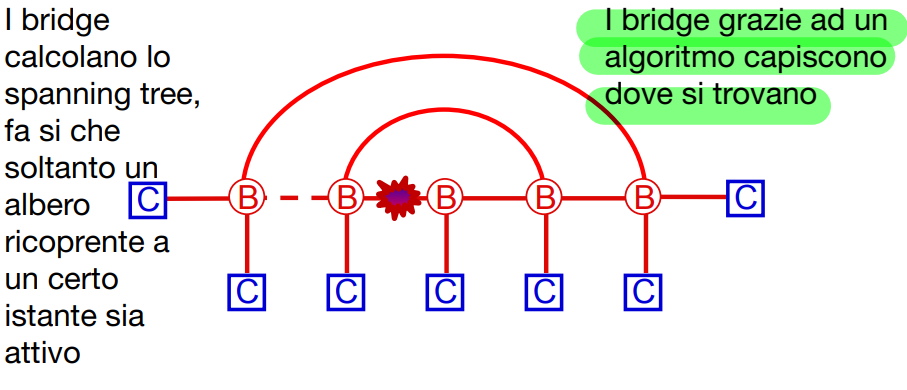
\includegraphics[width=13cm, height=6cm]{immagine_2024-12-26_163538431.png} % Percorso dell'immagine
    \caption{} % Didascalia per l'immagine
    \label{fig:immagine} % Etichetta per riferimento
\end{figure}
\noindent
\subsection{Altre informazioni}
Le prestazioni dei bridge influenzano le prestazioni dell'intera rete locale, tra i parametri che caratterizzano un bridge troviamo: numero massimo di pacchetti al secondo processabili e tempo medio di latenza: tempo di attraversamento del bridge da parte di un pacchetto, è preferibile che un bridge sia \textbf{full speed} ovvero i parametri sono pari al massimo teorico. Difficoltà sostanziale è che più corti sono i pacchetti e più è alto il numero di decisioni da prendere nell'unità di tempo.\\
L'amministratore di rete può mettere ogni porta in stato di \textbf{enabled} o \textbf{disabled}. Una porta attiva può essere in stato di \textbf{forwarding} o di \textbf{blocking}, a causa dell'algoritmo di spanning tree. Le porte hanno un indirizzo MAC e sono numerate progressivamente nel bridge a partire da 1, l'indirizzo del bridge è uguale all'indirizzo MAC della porta 1. Lo sviluppo di Ethernet ha portato all'uso di meccanismi di controllo di flusso, che servono sostanzialmente a non far andare lo switch in saturazione. A tal proposito si utilizza il pause frame che serve a regolare il flusso dei dati in una rete Ethernet, evitando che un dispositivo trasmetta più dati di quanti il dispositivo ricevente possa gestire.\\
\textbf{NOTA:} la latenza, è il tempo che ci mette un pacchetto ad attraversare l'intera rete, il ritardo di propagazione è il tempo che ci mette un bit per passare da un apparato all'altro.
\section{Reti locali senza fili o con pochi fili}
\subsection{Reti ad hoc}
Nelle Reti ad hoc le stazioni comunicano direttamente l'una con l'altra, il difetto principale e che si possono collegare pochi calcolatori
\subsection{Reti strutturate}
Nelle reti strutturate le stazioni comunicano l'una con l'altra solo mediante punti di accesso (Access Point o AP). Gli Access Point sono tutti collegati tra loro tramite una rete Wired. Un AP ha il MAC IEEE 802.11 e si comporta come un bridge. Ciscun AP controlla un BSS (Basic Service Set) e ognuno ha un identificatore (BSSID) infatti a tutti i PC collegati viene attribuito l’indirizzo MAC della scheda wireless dell’AP. Un altro elemento è DS (Distribution System) che è la rete wired (linea orizzontale del disegno) di backbone. È previsto anche il caso in cui gli AP (tutti o alcuni) comunichino wireless e non tramite l’infrastruttura wired.
\subsection{Il MAC (IEEE 802.11 WI-FI)}
Il MAC ha due algoritmi: quello che gestisce l’accesso distribuito al mezzo trasmissivo detto DCF (Distributed Coordination Function) e quello che gestisce l’accesso centralizzato al mezzo trasmissivo realizzato dal PCF (Point Coordination Function) (poco utilizzato).\\
In un pacchetto MAC ci sono vari campi:\\
\textbf{Frame control}: indica il tipo di pacchetto (di controllo o contenente dati). All'interno troviamo from e to DS, informazioni per la frammentazione e informazioni sulla riservatezza.\\
\textbf{Duration}: indica il tempo necessario per la trasmissione.\\
\textbf{Indirizzi}: contiene fino a 4 indirizzi tra cui mittente e destinatario più due bit, chiamati ToDS e FromDS, ToDS vale 1 quando il pacchetto è spedito all’AP per essere smistato sul DS. FromDS vale 1 quando il pacchetto è stato ricevuto dal DS\\
\textbf{Sequence control}: contiene informazioni utili per la frammentazione/riassemblaggio\\
\textbf{Body}: contiene una LLC-pdu o informazioni di controllo del MAC (dati da trasmettere)\\
\textbf{FCS}: 32 bit di crc (codice a ridondanza ciclica)
\subsection{Indirizzamento}
Ogni scheda wireless è dotata di un indirizzo MAC. Il pacchetto viene raccolto da una scheda wireless se è diretto al suo indirizzo MAC, ovviamente le macchine per scambiarsi pacchetti devono conoscere i corrispettivi indirizzi MAC. \textbf{Address 1} è sempre l’indirizzo MAC della scheda wireless a cui è destinato il pacchetto. \textbf{Address 2} è sempre l’indirizzo MAC della scheda wireless che trasmette il pacchetto. \textbf{Address 3} se FromDS=1 contiene SA se ToDS=1 contiene DA. \textbf{Address 4} è usato solo nel caso di comunicazione wireless nel distribution system. (Vedi esempi sulle slide e prova a farli).
\subsection{DCF (Distributed Coordination Function)}
Si occupa di: evitare interferenze tra trasmissioni simultanee (collisioni). DCF a sua volta utilizza l’algoritmo distribuito (In funzione contemporaneamente su più macchine) csma/ca: carrier sense multiple access / collision avoidance, se una stazione ha un pacchetto da spedire verifica se il mezzo trasmissivo è disponibile, se il mezzo trasmissivo è inutilizzato allora trasmette, altrimenti attende che la trasmissione corrente sia stata completata. È comunque possibile che due stazioni provino a trasmettere contemporaneamente: in questo caso si verifica una collisione e i pacchetti trasmessi diventano non intellegibili per i destinatari, i pacchetti che collidono sono ritrasmessi. DCF sfrutta gli intervalli tra pacchetti consecutivi come strumento per gestire delle priorità detti inter-packet gap. I due tipi principali sono \textbf{SIFS Short Inter-Frame Space ($SIFS<DIFS$)} e \textbf{DIFS DCF Inter-Frame Space}
\subsection{DCF senza RTS/CTS}
Quando una stazione vuole trasmettere ma il canale è occupato sceglie un numero random (detto di backoff) nell’intervallo $[0,cw]$ ed inizializza un timer, decrementa il timer di backoff mentre il canale è libero, quando il canale è occupato il decremento è sospeso, quando il timer raggiunge 0 la trasmissione può avvenire. Quando una stazione rileva una collisione duplica cw. Se un pacchetto è inviato con successo $cw=cw_{min}$. La trasmissione avviene quindi cosi:
\begin{figure}[H] % Usa 'H' per forzare la posizione qui
    \centering % Centra l'immagine
    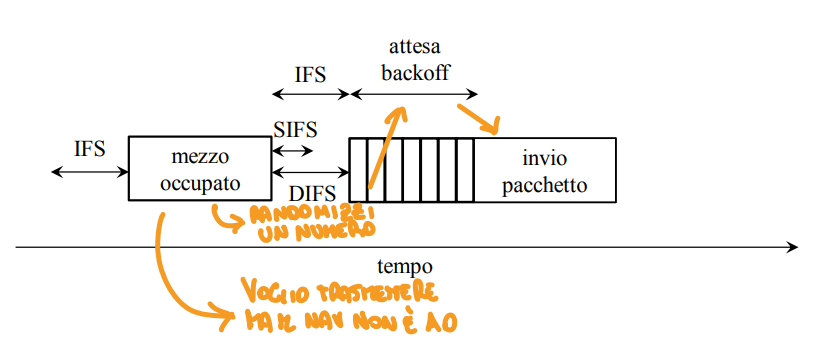
\includegraphics[width=14cm, height=5cm]{immagine_2024-12-27_132952681.png} % Percorso dell'immagine
    \caption{} % Didascalia per l'immagine
    \label{fig:immagine} % Etichetta per riferimento
\end{figure}
\noindent
In ogni pacchetto spedito (diverso da un ack) è specificata la durata (campo duration) della trasmissione ("Trasmetto per 20ns" gli altri nella rete sanno che il canale di trasmissione è occupato per 20ns). La durata viene memorizzata, da ogni stazione in ascolto, nel proprio \textbf{NAV (Network Allocation Vector)}. Il NAV viene utilizzato per sincronizzare le stazioni, infatti, ogni stazione decrementa il suo NAV con il passare del tempo, una stazione può trasmettere solo quando il proprio NAV è zero.
\begin{figure}[H] % Usa 'H' per forzare la posizione qui
    \centering % Centra l'immagine
    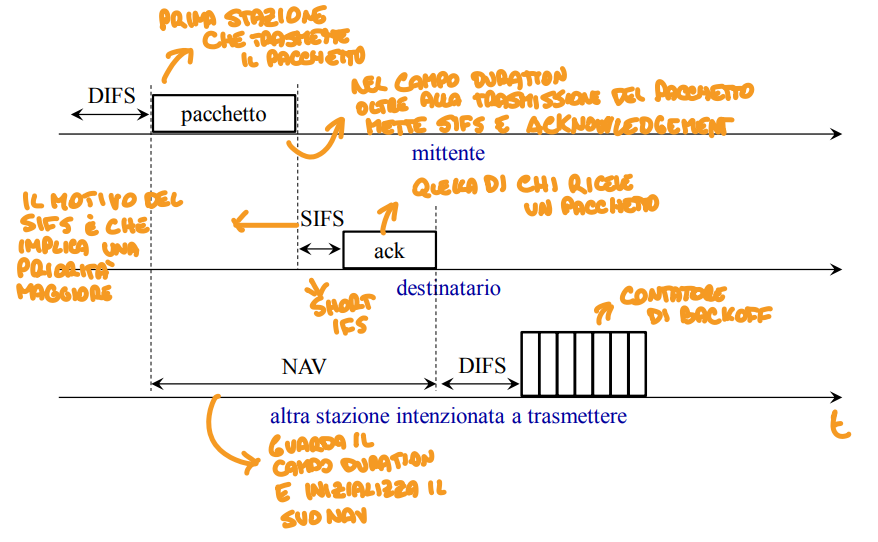
\includegraphics[width=14cm, height=5cm]{immagine_2024-12-27_133455594.png} % Percorso dell'immagine
    \caption{} % Didascalia per l'immagine
    \label{fig:immagine} % Etichetta per riferimento
\end{figure}
\noindent
I pacchetti sono riscontrati per mezzo di acknowledgement (ack): la stazione destinataria, se riceve il pacchetto correttamente, invia sempre un riscontro (ack) al mittente. Nella spedizione di un acknowledgement si attende SIFS.\\
Il MAC IEEE 802.11 usa due strumenti per fare verificare la disponibilità del canale (per fare carrier sense) \textbf{fisico}: informazione di canale libero dal livello fisico (vede se sul canale trasmissivo c'è del segnale attivo) e \textbf{logico}: il NAV. Il canale è libero se il livello fisico segnala libero e se il NAV è a 0. Una \textbf{collisione} si verifica quando un pacchetto non ottiene ack.
\subsection{DCF con RTS/CTS}
CI sono due problemi che vanno affrontati: se il pacchetto su cui si verifica una collisione è molto grande, si perde molto tempo prima che la collisione sia identificata, nelle reti wireless è possibile che tra le stazioni ci sia visibilità parziale.
\subsection{Trasmissione con uso di RTS (Request To Send)/ CTS (Clear To Send)}
Quando una stazione vuole trasmettere spedisce un breve frame al destinatario, chiedendo l'autorizzazione alla trasmissione. Se il destinatario è disponibile emette un breve frame di conferma, alle stazioni vicine è richiesto di non interferire per l'intera durata della trasmissione che sta per avvenire. Quindi:
\textbf{A} vuole trasmettere a \textbf{B} ed il canale è libero. \textbf{A} manda un RTS (Request To Send) a \textbf{B}. \textbf{B} è libero quindi manda un CTS (Clear To Send) a \textbf{A}. Tutte le stazioni che ricevono il CTS inviato da \textbf{B} e/o l'RTS inviato da \textbf{A}, ora sanno che \textbf{B} ed \textbf{A} stanno trasmettendo. Le stazioni che vogliono trasmettere ad \textbf{A} o \textbf{B} dovranno aspettare un tempo pari alla "duration" specificata nei pacchetti inviati da \textbf{A} o \textbf{B}. \textbf{A} trasmette a \textbf{B}. Le uniche \textbf{collisioni} possibili sono dovute all'invio simultaneo dell'RTS da parte di due stazioni, non viene quindi ricevuto un CTS.\\\\
\textbf{Sintesi Backoff:}
Una stazione che rileva una collisione o che trova il canale occupato sceglie un numero a caso tra 0 e cw, il numero viene moltiplicato per un tempo chiamato slot- time e viene inizializzato il timer di attesa per backoff. Ad ogni nuova collisione sullo stesso pacchetto l’estremo superiore della cw viene raddoppiato fino ad un massimo di $c_{max}$, per ogni slot-time (intervallo di tempo) che il canale rimane
libero, il timer viene decrementato di uno slot-time, il valore viene decrementato solamente se il canale è libero (cioè se il NAV della stazione è pari a zero), quando il timer è a zero la stazione può trasmettere, quando una trasmissione ha successo cw è riportato a $cw_{min}$\\\\
Nella pratica nelle stazioni è definita una soglia s che stabilisce per quali pacchetti utilizzare RTS/CTS.
\subsection{Handshaking}
L'insieme delle stazioni di un BSS (Guarda slide se non ricordi 54 insieme verde scuro) cambia continuamente (computer accesi, spenti...). Una stazione che vuole accedere a un BSS deve scambiare informazioni di \textbf{handshaking} con l'AP di quel BSS. AP e stazione presentano i propri indirizzi MAC. Per \textbf{accedere} a un BSS ci sono due possibilità, l'utilizzo di pacchetti "beacon" (faro) inviati dall'AP o l'utilizzo di pacchetti "probe" (sonda) inviati dalla stazione.
\subsection{Reti logiche}
Un amministratore può definire varie reti logiche sulla stessa rete fisica ciascuna identificata da un SSID ( Service Set ID ). Un AP con un BSSID può, attraverso i suoi annunci, dirsi disponibile a far passare il traffico di uno o più SSID.
\subsection{IEEE 802.11 Frammentazione}
Il livello MAC può decidere di frammentare un pacchetto. Frammentare può essere utile per avere pacchetti di dimensioni inferiori alle LAN cablate, per ridurre l'overhead in caso di ritrasmissione del pacchetto e per ridurre la probabilità di errore nella trasmissione. \textbf{Ciascun} frammento viene trattato come un pacchetto (MAC hdr, body, crc) e viene riscontrato singolarmente. Il MAC ricevente riassembla i frammenti ricostruendo il pacchetto.\\\\
Trasmissioni verso l'indirizzo MAC broadcast: Nel caso in cui ToDS = 0 non si usano ack e non si usano RTS/CTS (le collisioni non sono rilevate). Nel caso in cui ToDS = 1 si usano ack ed eventualmente RTS/CTS (i pacchetti vanno verso l'AP), è possibile configurare un AP in modo tale che un pacchetto broadcast ricevuto sia o meno inviato a tutto il BSS.
\section{Reti di raccolta e Reti di accesso}
Vi è una zona intermedia tra LAN e WAN che è costituita da una rete di raccolta e una rete di accesso.
\subsection{Rete di raccolta}
\textbf{FTTN (Fiber To The Node)} e \textbf{FTTC (Fiber To The Cabinet)} sono i metodi di raccolta più comuni e corrispondono alle tecnologie conosciute come xDSL (xDigital Subscriber Line) (al posto della x possono esserci varie lettere a seconda di alcuni parametri come la banda) \\
\textbf{FTTB (Fiber To The Building)} e \textbf{FTTH (Fiber To The Home)} sono i metodi di raccolta in corso di realizzazione e sono in grado di garantire linee a più di 1Gbit/sec; fanno uso di OLT (GPON) (vedi slide 5 per chiarimenti). \textbf{GPON (Gigabit-capable Passive Optical Network)} è una tecnologia per la raccolta del traffico dei clienti, fa uso di apparati chiamati OLT (Optical Line Termination), sui quali arrivano le fibre ottiche dei clienti, un OLT è essenzialmente uno switch in cui su ogni porta possono essere collegati fino a 64 clienti. Nello splitting ottico i dispositivi non devono essere alimentati da corrente ma mettono assieme dati di diversi clienti.

\subsection{La rete di accesso}
Tra la rete di raccolta e la WAN c'è la rete di accesso. È una rete di switch con un'estensione geografica significativa, tuttavia non può essere troppo grande perchè vogliamo evitare che ci siano switch a cascata uno dentro l'altro, viene anche chiamata \textbf{MAN (Metro Area Network)}.\\
Per rispondere ai requisiti prestazionali e di manutenibilità l'architettura è molto semplice. Ed è composta da switch connessi in un anello, questo risulta utile per la ridondanza, infatti, in caso si rompa qualcosa la rete continuerebbe a funzionare. Gli switch non restano accesi tutti contemporaneamente ma resta acceso soltanto lo spanning tree.
\subsection{Architettura delle reti di accesso}
\begin{figure}[h]
    \centering
    \begin{minipage}{0.4\textwidth} % Imposta la larghezza della colonna sinistra
        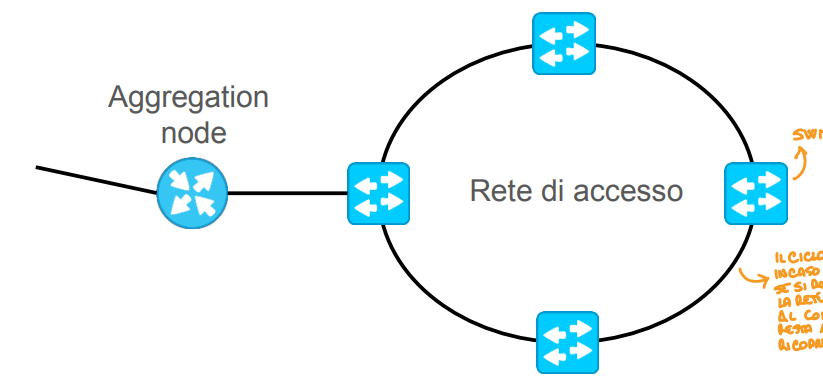
\includegraphics[width=7cm,height=4cm]{immagine_2024-12-27_150634942.png}
       % \caption{Architettura delle reti di accesso} % Opzionale
        \label{fig:immagine}
    \end{minipage}%
    \hfill
    \begin{minipage}{0.55\textwidth} % Imposta la larghezza della colonna destra
        Un \textbf{aggregation node} collega la rete di accesso al backbone (WAN) del provider. Se si rompe uno switch, solo i clienti attestati su quello switch hanno un disservizio. Per aumentare la robustezza dell'anello spesso si realizzano doppi collegamenti.
    \end{minipage}
\end{figure}
\section{Metodi e modelli per il livello di rete}
\subsection{Il livello di rete}
Il \textbf{livello di rete} sceglie una strada per i pacchetti, la strada verso la destinazione è composta da vari passaggi intermedi (salti o hop). Il livello di rete \textbf{fornisce servizi} al livello di trasporto, il quale non è interessato a conoscere: il numero e la topologia delle varie reti, che vengono attraversate per raggiungere una destinazione e le tecnologie di livello inferiore usate per realizzare le reti attraversate. I servizi offerti dal livello di rete al livello di trasporto possono essere \textbf{connessi} (il che prevede un dialogo tra dispositivi con dei riscontri) o \textbf{non connessi}. L'instradamento può essere a datagramma o a circuito virtuale. Un livello di rete connesso fa tipicamente uso della commutazione a circuito virtuale mentre uno non connesso fa uno della commutazione a datagramma.\\\\
Dal punto di vista del livello 3 i sistemi sulla rete possono essere: \textbf{End System (es)} o \textbf{Intermediate System (is)}. A ogni sistema viene associato un indirizzo numerico e un nome, informazioni sulla corrispondenza nomi-indirizzi sono gestite da server appositi, chiamati name server. Gli is, chiamati anche router o gateway, operano a livello 3 e contengono gli strati 1, 2 e 3 dell'architettura ISO-OSI. Vi è bisogno di trovare un modo per far corrispondere gli indirizzi di livello 2 (MAC) con gli indirizzi di livello 3 (identificatore nell'intera rete). Infatti un sistema necessita di tanti indirizzi MAC quante sono le sue schede di rete e di un solo indirizzo di livello 3.
\subsection{Metodi di instradamento}
Gli is possono effettuare instradamento con tre metodi principali:\\\\
\textbf{Routing by network address}
\begin{figure}[H]
    \centering
    \begin{minipage}{0.55\textwidth} % Imposta la larghezza della colonna sinistra
        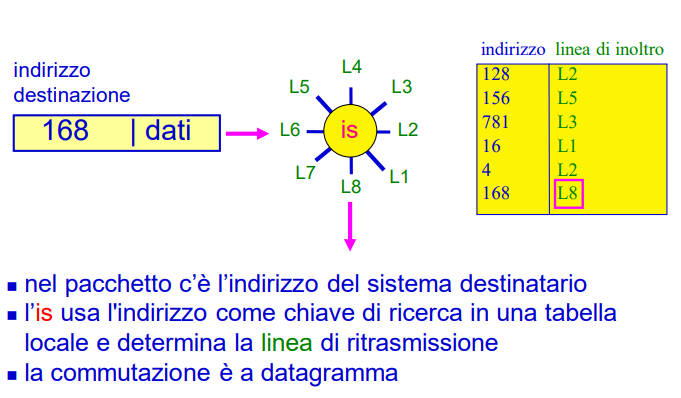
\includegraphics[width=9cm,height=5cm]{immagine_2024-12-28_144229637.png}
        %\caption{Routing by network address} % Opzionale
        \label{fig:immagine}
    \end{minipage}%
    \hfill
    \begin{minipage}{0.45\textwidth} % Imposta la larghezza della colonna destra
        Questo metodo è valido indipendentemente da chi compila la tabella. Se l'indirizzo non fosse presente nella tabella il pacchetto verrebbe buttato, al contrario di uno switch che l avrebbe mandato a tutti. La tabella di un is che fa routing by network address contiene l'elenco di tutti gli indirizzi presenti nella rete.
    \end{minipage}
\end{figure}
\noindent
\textbf{Label (senza) swapping}
\begin{figure}[H]
    \centering
    \begin{minipage}{0.55\textwidth} % Imposta la larghezza della colonna sinistra
        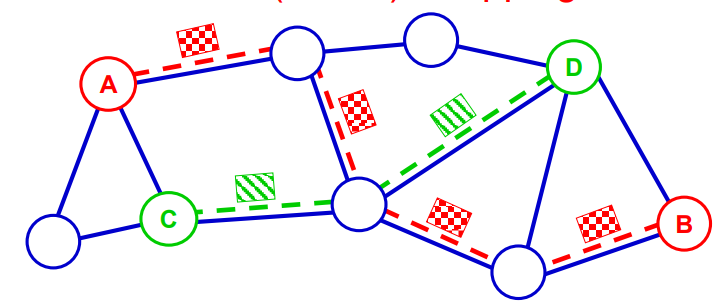
\includegraphics[width=9cm,height=5cm]{immagine_2024-12-28_144440892.png}
        %\caption{Label (senza) swapping} % Opzionale
        \label{fig:immagine}
    \end{minipage}%
    \hfill
    \begin{minipage}{0.45\textwidth} % Imposta la larghezza della colonna destra
       La commutazione è a circuito virtuale. Nel pacchetto c'è un eticchetta che identifica il circuito virtuale. Ogni is usa la label come chiave di ricerca in una tabella locale, molto piccola, e determina la linea di ritrasmissione. Quello che notiamo è che i pacchetti vengono colorati e avranno un colore che identifica il percorso, questo serve a far capire agli is dove mandare il pacchetto. La tabella di un is che fa label swapping contiene l'elenco dei circuiti virtuali che lo attraversano in un certo istante.
    \end{minipage}
\end{figure}
\vspace{200pt}
\noindent
\textbf{Label swapping}
\begin{figure}[H]
    \centering
    \begin{minipage}{0.55\textwidth} % Imposta la larghezza della colonna sinistra
        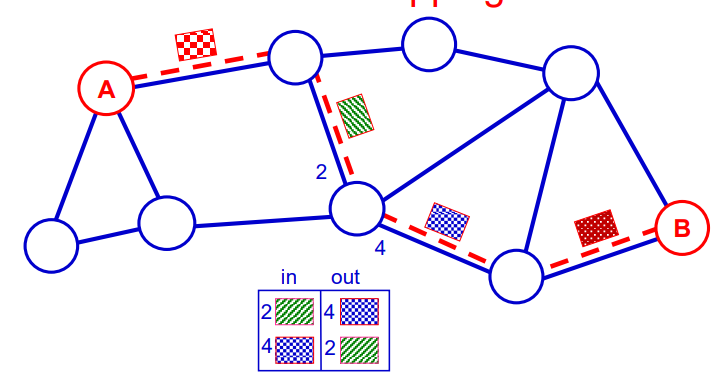
\includegraphics[width=9cm,height=5cm]{immagine_2024-12-28_145027694.png}
        %\caption{Label swapping} % Opzionale
        \label{fig:immagine}
    \end{minipage}%
    \hfill
    \begin{minipage}{0.45\textwidth} % Imposta la larghezza della colonna destra
      Per evitare di dover verificare nell'intera rete che una specifica label non sia già utilizzata per qualche altra connessione, ad ogni tratto del circuito è assegnata una label (in generale) diversa ed assegnata localmente. In questo modo la label può essere scelta localmente dagli is che condividono il link
    \end{minipage}
\end{figure}
\noindent
\textbf{Source Routing}
\begin{figure}[H]
    \centering
    \begin{minipage}{0.55\textwidth} % Imposta la larghezza della colonna sinistra
        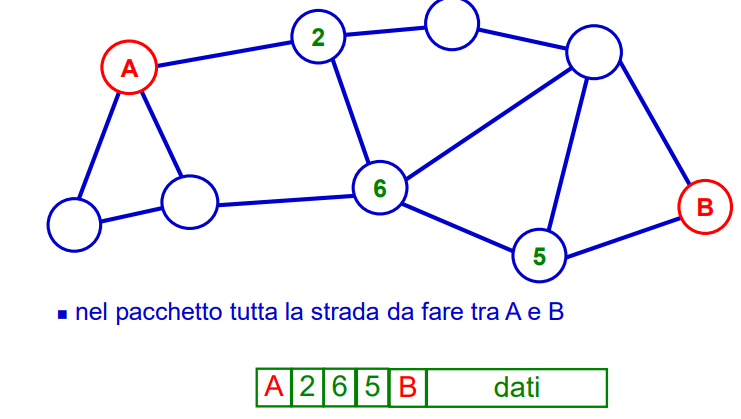
\includegraphics[width=9cm,height=5cm]{immagine_2024-12-28_145210897.png}
        %\caption{Source Routing} % Opzionale
        \label{fig:immagine}
    \end{minipage}%
    \hfill
    \begin{minipage}{0.45\textwidth} % Imposta la larghezza della colonna destra 
    \end{minipage}
\end{figure}
\noindent
Un router ha quindi due funzioni, che sono \textbf{control plane} dove esegue l'algoritmo di calcolo della tabella di instradamento e \textbf{data plane} dove guarda la tabella di instradamento e fa un azione sul pacchetto tramite il processo di forwarding.
\section{IPv4, ARP e la suite TCP/IP}
Il protocollo \textbf{IPv4 (Internet Protocol versione 4)} è il principale protocollo di rete (di livello 3) della "suite TCP/IP", detta anche "Internet Protocol Suite". La \textbf{suite TCP/IP} è la pila protocollare usata in Internet. Tra i suoi obiettivi troviamo semplificare il data plane degli is e spostare tutte le funzioni complesse sugli es.
\subsection{IPv4}
Insieme a IPv6 è il principale protocollo di lvl3. I suoi \textbf{pacchetti} vengono anche detti \textbf{IPv4 datagram}, questo protocollo si occupa di instradare, frammentare, riassemblare e rilevare gli errori. Riceve messaggi dai protocolli \textbf{UDP e TCP} del livello superiore. La dimensione dei datagram dipende dai vincoli di lvl 2, infatti se il datagram è troppo grande, IPv4 provvede alla frammentazione.
\subsubsection{IPv4 Datagram}
Analogamente ai pacchetti di lvl 2, il datagram IPv4 è diviso in due parti: l'\textbf{header} e i \textbf{dati}. L'header contiene gli indirizzi del mittente e del destinatario.
\begin{figure}[H] % Usa 'H' per forzare la posizione qui
    \centering % Centra l'immagine
    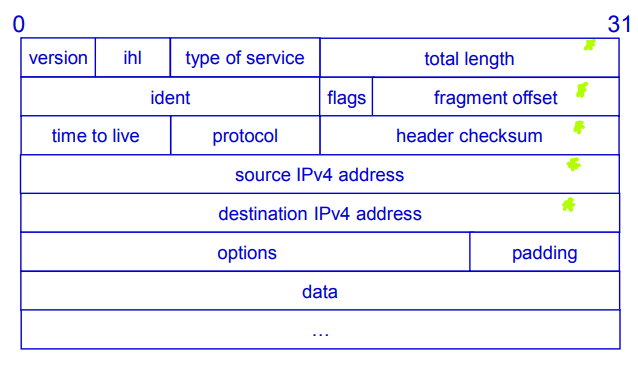
\includegraphics[width=14cm, height=5cm]{Screenshot 2024-12-28 152140.png} % Percorso dell'immagine
    \caption{Datagram Header} % Didascalia per l'immagine
    \label{fig:immagine} % Etichetta per riferimento
\end{figure}
\noindent
\textbf{Version}: è la versione del protocollo IP che ha generato il pacchetto, attualmente vale 4.\\
\textbf{Ihl} è la lunghezza dell'header, espressa in parole da 32 bit (4 byte).\\
\textbf{Type of Service}: specifica la priorità di un datagram rispetto a un altro.\\
Prima di introdurre i campi \textbf{ident, flags e fragment offset} è necessario capire perchè frammentare i pacchetti a livello 3. Sostanzialmente potrebbero capitarci due situazioni: ogni livello due attraversato potrebbe avere una \textbf{maximum transmission unit (mtu)} (dimensione massima di un pacchetto diversa), il pacchetto di livello tre potrebbe essere troppo grande per essere imbustato in un pacchetto data link intermedio. La \textbf{frammentazione} consiste nella suddivisione di un pacchetto in pacchetti più piccoli. Il \textbf{riassemblaggio} consiste nella ricostituzione del pacchetto sulla macchina destinazione. Infatti a tal proposito occorrono i campi nell'header di livello tre che consentano di: riconoscere il pacchetto come frammento, riconoscere i frammenti generati dallo stesso pacchetto, determinare l'ordine dei frammenti in maniera da poter riassemblare il pacchetto originale. L'adozione di un offsett consente la eventuale successiva frammentazione dei frammenti. Infatti:\\
\textbf{Ident}: è un intero che identifica un datagramma, serve all'IPv4 dell'host ricevente nel momento del riassemblaggio. Due datagrammi con lo stesso ident vengono riassemblati nello stesso pacchetto.\\
\textbf{Fragment Offset}: serve a riunire i frammenti nel giusto ordine. Essendo di 13 bit, può specificare solo un offset multiplo di 8 ( con la convenzione che gli ultimi tre bit siano zeri).\\
\textbf{Flags}: Il primo bit è riservato e deve essere sempre 0. \textbf{DF (Don't fragment)} specifica se il datagram può essere frammentato. \textbf{MF (more fragment)} permette di riconoscere l'ultimo frammento del pacchetto (slide 22 per chiarezza sulla frammentazione).\\
\textbf{Total Length}: è la lunghezza del pacchetto completo di header e payload.\\
\textbf{Time to Live}: specifica il tempo di vita del pacchetto, viene decrementato con il passare del tempo, quando il pacchetto vale 0 viene scartato, quando il pacchetto è scartato il router manda un avvertimento al mittente.\\
\textbf{Protocol}: identifica il protocollo di livello superiore che è nel payload del pacchetto IPv4.\\
\textbf{Header checksum}: riguarda solo l'header, deve essere ricalcolato a ogni hop.\\
\textbf{Options}: è usato per specificare informazioni meno frequenti nei pacchetti.
\subsubsection{Indirizzamento IPv4}
Gli indirizzi sono associati alle schede di rete e non agli host. Gli indirizzi sono di 32 bit, univoci a livello mondiale e per comodità si rappresentano con 4 numeri decimali separati da punti. Ovviamente se gli indirizzi IPv4 fossero assegnati in modo del tutto arbitrario la tabella di instradamento di un router dovrebbe contenere un numero enorme di righe. La soluzione è quella di assegnare indirizzi che cominciano nello stesso modo a macchine allocate fisicamente nella stessa rete locale. Un gruppo di macchine è quindi individuato dallo stesso prefisso, un is conterrà tabelle di prefissi invece che tabelle di indirizzi. Gli indirizzi delle macchine di una stessa rete fisica appartengono a una stessa \textbf{net}. Nei primi anni di Internet sono state definite cinque classi di indirizzi con prefissi di diversa lunghezza. Le classi sono: A, B, C, D, E. Dato un indirizzo si poteva inferire la sua classe di appartenenza esaminandone solo i primi bit.
\begin{figure}[H] % 'h' per indicare di posizionare la figura qui
    \centering % Centra l'intera figura
    % Immagine di sinistra
    \begin{subfigure}[t]{0.45\textwidth} % Sottotitolo di dimensione 45% della larghezza
        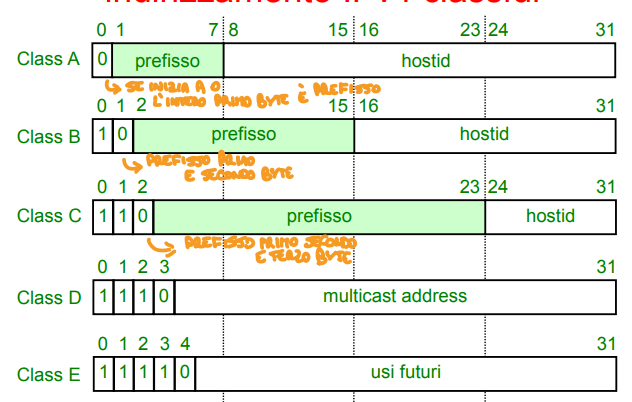
\includegraphics[width=\linewidth]{Screenshot 2024-12-28 155856.png} % Percorso dell'immagine
       % \caption{Arrivo in precedenza dei processi più piccoli} % Didascalia per la prima immagine
        \label{fig:sinistra} % Etichetta per riferimento
    \end{subfigure}
    \hspace{0.05\textwidth} % Spazio orizzontale tra le immagini
    % Immagine di destra
    \begin{subfigure}[t]{0.45\textwidth} % Sottotitolo di dimensione 45% della larghezza
        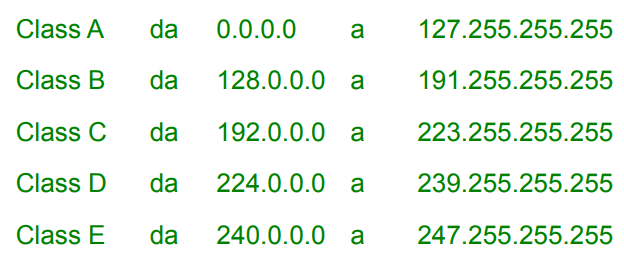
\includegraphics[width=\linewidth]{Screenshot 2024-12-28 155906.png} % Percorso dell'immagine
       % \caption{Arrivo in precedenza del processo più grande} % Didascalia per la seconda immagine
        \label{fig:destra} % Etichetta per riferimento
    \end{subfigure}
   % \caption{SJF/Shortest Job First} % Didascalia generale per la figura
    \label{fig:due_immagini} % Etichetta generale per riferimento
\end{figure}
\noindent
L'indirizzamento classful è stato abbandonato per consentire una lunghezza arbitraria dalla parte prefisso dell'indirizzo IPv4 (indirizzamento classless). Ad ogni indirizzo IPv4 viene associata una \textbf{netmask}: sequenza di 32 bit, composta da uno contigui seguiti da zeri. Gli uno rappresentano i bit del prefisso, mentre l host è identificato dai restanti bit. La netmask di un prefisso si può denotare più semplicemente specificando, dopo l'indirizzo IPv4, la lunghezza del prefisso, separata da una barra.
\subsubsection{Invio di un pacchetto}
La configurazione delle interfacce degli es prevede, oltre all'assegnazione di un indirizzo IPv4, anche la specifica della netmask della net di appartenenza. Mettendo in and-bit-a-bit il proprio indirizzo e quello del destinatario con la propria netmask, l'es determina se un destinatario è locale o remoto. Se il destinatario è locale il pacchetto viene inviato al destinatario stesso (trasmissione diretta), se il destinatario è remoto il pacchetto viene inviato al \textbf{default gateway} della LAN, cioè a un router (un is). (Esempio slide 41).
\subsubsection{Indirizzamento IPv4 classless - IP Lookup}
La ricerca nella tabella di instradamento (IP lookup) funziona: ogni riga della tabella di instradamento di un router contiene un prefisso e la relativa netmask. Per ogni riga, mettendo in and bit-a-bit l'indirizzo IPv4 del destinatario con la netmask e confrontandolo con prefisso il router determina se l'indirizzo è nella LAN relativa. La tabella viene controllata una riga dopo l'altra. Non appena si riscontra un matching il pacchetto viene inoltrato sulla linea relativa. Se non avviene nessun matching il pacchetto viene scartato. La riga 0.0.0.0/0 viene chiamata \textbf{rotta di default}, produca matching con qualsiasi indirizzo.
\subsubsection{Tabelle di instradamento}
Abbiamo visto tutti gli elementi delle tabelle di instradamento manca solo un ultimo elemento, il \textbf{next hop}. Sostanzialmente si manda il pacchetto a un'altro router che proseguirà il cammino. Un altra cosa che abbiamo visto è l'indirizzo di \textbf{loopback} il quale serve a farci "rimbalzare" il pacchetto per far comunicare due applicazioni sulla stessa macchina.
\subsection{ARP}
Il protocollo \textbf{ARP} ci permette di capire quale indirizzo MAC corrisponde a un certo indirizzo IPv4. Sostanzialmente funziona cosi: l'host invia un messaggio broadcast a tutti gli host di una rete, nel quale chiede alle macchine l'indirizzo MAC corrispondente all'indirizzo IPv4 dato (\textbf{ARP request}). L'host che ha quell'indirizzo IPv4 risponde con \textbf{ARP reply}, fornendo il proprio MAC. Gli host che usano ARP hanno a disposizione una cache in cui memorizzano le corrispondenze IPv4-MAC di cui sono venuti a conoscenza. Solo se l'indirizzo IPv4 non viene trovato nella "ARP cache" si procede ad inviare in broadcast una ARP request. I messaggi ARP vengono spediti da una macchina all'altra incapsulati nel campo  dati del pacchetto di livello 2.
\begin{figure}[H] % Usa 'H' per forzare la posizione qui
    \centering % Centra l'immagine
    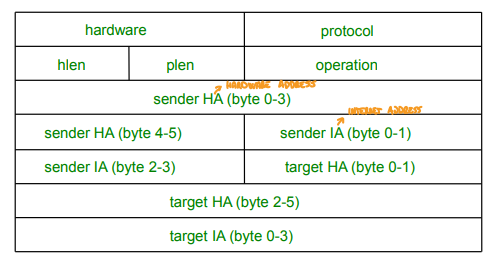
\includegraphics[width=10cm, height=4cm]{immagine_2024-12-28_171110557.png} % Percorso dell'immagine
   % \caption{Datagram Header} % Didascalia per l'immagine
    \label{fig:immagine} % Etichetta per riferimento
\end{figure}
\noindent
I campi \textbf{hardware e protocol} specificano il tipo di indirizzo di livello 2 e il tipo di indirizzo di livello 3. I campi \textbf{hlen e plen} specificano la lunghezza dei due indirizzi. Nel campo \textbf{operation} si specifica se il messaggio è una ARP request o una ARP reply. I campi \textbf{sender ia e ha} sono rispettivamente l'indirizzo di livello 3 e di livello 2 del mittente. Il campo \textbf{target ia} contiene l'indirizzo di livello 3 della macchina di cui si vuole conoscere l'indirizzo di livello 2 nel caso di un ARP request. 
\section{Il protocollo ICMP (per IPv4) e i comandi ping e traceroute}
Il protocollo IPv4 ha un approccio \textbf{best effort} (sforzo migliore): non è in grado di garantire la consegna dei pacchetti, ma esegue dei tentativi, al meglio delle possibilità di cui dispone. Alcuni pacchetti possono essere scartati da IPv4: sono "dropped on the floor". \textbf{ICMP (Internet Control Message Protocol)} offre, a supporto di IPv4, un semplice servizio di \textbf{error-reporting}, consente inoltre di spedire messaggi per richiedere, ed eventualmente ottenere, informazioni. \textbf{HOP}, un computer intermedio tra la sorgente e la destinazione del pacchetto.
ICMP ha principalmente \textbf{3 regole}: nessun messaggio ICMP viene generato a seguito di eventuali errori rilevati su altri messaggi ICMP, se il pacchetto viene frammentato, allora solo il primo frammento può generare messaggi di errore ICMP, i pacchetti broadcast e multicast non generano ICMP.
\begin{figure}[H] % Usa 'H' per forzare la posizione qui
    \centering % Centra l'immagine
    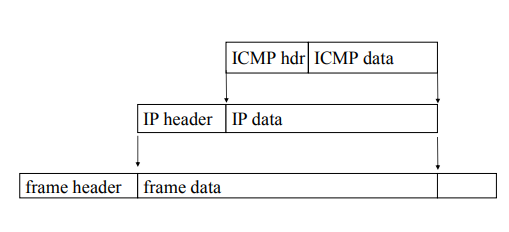
\includegraphics[width=10cm, height=4cm]{Screenshot 2024-12-30 111559.png} % Percorso dell'immagine
   % \caption{Datagram Header} % Didascalia per l'immagine
    \label{fig:immagine} % Etichetta per riferimento
\end{figure}
\noindent
\subsection{Tipi di messaggi}
\subsubsection{Messaggi di destination unreachable}
\textbf{Network Unreachable}: un gateway vede la rete a cui è destinato il pacchetto a distanza infinita.\\
\textbf{Host Unreachable}: l'host a cui è destinato il pacchetto non risponde ad una chiamata ARP.\\
\textbf{Protocol Unreachable}: l'host a cui è destinato il pacchetto non conosce il protocollo nel pacchetto.\\
\textbf{Port Unreachable}: la port specificata non è raggiungibile.\\
\textbf{Fragment needed and DF set}: il pacchetto non può essere frammentato.
\subsubsection{Messaggi di tempo scaduto}
\textbf{TIME\_EXCEEDED (tempo scaduto)}: il pacchetto ha TTL=0 e quindi viene scartato
\subsubsection{Messaggi di redirection}
\textbf{Redirect (ridireziona)}: un router rileva che il prossimo router a cui dovrebbe inoltrare il pacchetto è sulla stessa LAN del mittente.
\subsubsection{Messaggi di Eco}
\textbf{ECHO\_REQUEST e REPLY}: controllo di raggiungibilità di un host\\
\textbf{TIMESTAMP e TIMESTAMP\_REPLY}: come ECHO, più informazioni sull'orario dell'invio. Misura la velocità del collegamento, sincronizzzazione (approssimativa) dell'ora di sistema.
\subsection{Il comando Ping}
Il comando \textbf{Ping} ha l'obiettivo di verificare se un indirizzo IP è raggiungibile e qual è il ritardo per raggiungerlo. Invia una sequenza di pacchetti \textbf{ICMP ECHO\_REQUEST} e attende la relativa risposta \textbf{ECHO\_REPLY}. Misura il tempo che intercorre tra l'invio della richiesta e la ricezione della risposta per ogni pacchetto. 
\subsection{Il comando Traceroute}
Il comando \textbf{Traceroute} ha l'obiettivo di verificare quali router sono attraversati per raggiungere un dato indirizzo IP. Sostanzialmente si invia un pacchetto con TTL molto basso, in modo che muoia e faccia in modo che il primo router attraversato mandi un time excited e si continua così aumentando progressivamente il TTL.
\section{Rappresentazione a albero IPv4}
Lo spazio degli indirizzi IPv4 può essere rappresentato mediante un'albero binario. Il bit associato all'arco rappresenta il bit più significativo. Per ciascun nodo il figlio sinistro è etichettato con uno 0 il destro con un 1. In questa rappresentazione, una \textbf{net} corrisponde ad un nodo non foglia \textbf{X} e al sottoalbero radicato a \textbf{X}. Le foglie del sottoalbero radicato a \textbf{X} corrispondono a tutti gli indirizzi della net. Il prefisso della net che corrisponde a \textbf{X} si ottiene concatenando le etichette degli archi attraversati nel cammino dalla radice a \textbf{X}. Le net con prefisso /y significano i nodi a distanza y dalla radice. Siano \textbf{A} e \textbf{B} due nodi che rappresentano due prefissi, se \textbf{A} è nel cammino dalla radice a \textbf{B} allora \textbf{A} contiene tutti gli indirizzi di \textbf{B}, il contrario viceversa. Siano \textbf{A} e \textbf{B} due nodi che rappresentano due prefissi \textbf{A} e \textbf{B} sono il subnetting (tagliare una net in due parti) esatto di \textbf{C} se e solo se \textbf{C} è il genitore di entrambi. Una \textbf{tabella di instradamento} è una lista di nodi dell'albero in cui ad ogni nodo della lista è associata un'interfaccia ed eventualmente un next hop.
\section{IPv6 e ICMPv6}
Gli indirizzi \textbf{IPv4} sono in rapido esaurimento. \textbf{IPv6} ha uno spazio di indirizzamento molto più ampio di IPv4.
\subsection{Header IPv6}
\begin{figure}[H] % Usa 'H' per forzare la posizione qui
    \centering % Centra l'immagine
    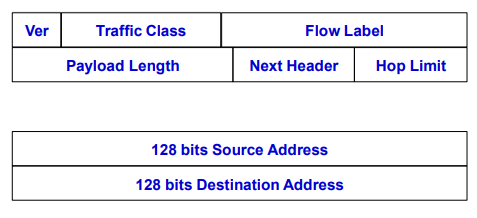
\includegraphics[width=10cm, height=4cm]{immagine_2025-01-02_112745553.png} % Percorso dell'immagine
   % \caption{Datagram Header} % Didascalia per l'immagine
    \label{fig:immagine} % Etichetta per riferimento
\end{figure}
\noindent
Spariscono le options.\\
\textbf{Version}: 6.\\
\textbf{Traffic Class}: simile al Type of Service di IPv4.\\
\textbf{Flow Label}: per distinguere un flusso. I pacchetti appartenenti allo stesso flusso hanno: stesso indirizzo IPv6 sorgente, stesso indirizzo IPv6 destinazione, stesso valore del campo flow-label.\\
\textbf{Payload Length}: specifica la lunghezza del campo dati nel pacchetto.\\
\textbf{Next Header}: simile a protocol di IPv4; consente anche di specificare le options.\\
\textbf{Hop Limit}: uguale al ttl di IPv4.\\
\textbf{Source address e Destination Address}\\
I campi che mancano sono quelli che non ci sono più, ovvero: \textbf{i campi per la frammentazione}, in IPv6 i router non possono frammentare i pacchetti. La frammentazione avviene solo sugli es, che devono scoprire, tramite un opportuno protocollo, la MTU minima di un path. \textbf{Checksum} si suppone che i controlli di livello 2 e di livello 4 siano sufficienti e \textbf{Hlen}, infatti l'header è di lunghezza fissa e ha sempre 40 byte.
\subsection{Rappresentazione degli indirizzi IPv6}
Un indirizzo IPv6 al contrario di IPv4, si rappresenta con 8 numeri esadecimali separati da due punti. Ogni numero esadecimale rappresenta 16 bit.
\begin{figure}[H] % Usa 'H' per forzare la posizione qui
    \centering % Centra l'immagine
    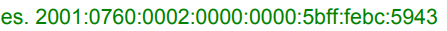
\includegraphics[width=14cm, height=1cm]{immagine_2025-01-02_113658978.png} % Percorso dell'immagine
   % \caption{Datagram Header} % Didascalia per l'immagine
    \label{fig:immagine} % Etichetta per riferimento
\end{figure}
\noindent
Talvolta la scrittura può essere semplificata togliendo i zeri meno significativi dai quartetti. 
\begin{figure}[H] % Usa 'H' per forzare la posizione qui
    \centering % Centra l'immagine
    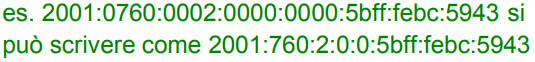
\includegraphics[width=14cm, height=1cm]{immagine_2025-01-02_113924536.png} % Percorso dell'immagine
   % \caption{Datagram Header} % Didascalia per l'immagine
    \label{fig:immagine} % Etichetta per riferimento
\end{figure}
\noindent
Inoltre è consentito omettere gruppi consecutivi (anche uno solo) di 16 bit contenenti solo zeri.
\begin{figure}[H] % Usa 'H' per forzare la posizione qui
    \centering % Centra l'immagine
    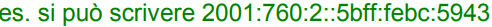
\includegraphics[width=14cm, height=1cm]{immagine_2025-01-02_114027668.png} % Percorso dell'immagine
   % \caption{Datagram Header} % Didascalia per l'immagine
    \label{fig:immagine} % Etichetta per riferimento
\end{figure}
\noindent
La notazione con i due punti consecutivi è utilizzabile una sola volta in un indirizzo.\\
0.0.0.0.0.0.0.1 si può scrivere ::1 e rappresenta l'interfaccia di \textbf{loopback} della macchina, analogo al 127.0.0.1 di IPv4. Per i \textbf{prefissi} si usa la stessa notazione con / usata in IPv4. Non ci sono prefissi più lunghi di una /64. Una netmask non è rappresentata nel formato in cui sono espliciti i valori dei suoi bit. 
\subsection{Indirizzi unicast e multicast}
Anche in IPv6 ci sono indirizzi unicast e multicast, ma non ci sono indirizzi broadcast. Gli indirizzi unicast più importanti sono: \textbf{indirizzi global unicast e indirizzi link-local}. Gli indirizzi multicast più importanti sono: \textbf{solicited node, ff02::1 (tutte le macchine della LAN), ff02::2 (tutti i router della LAN)}. Un indirizzo \textbf{unicast} è sempre formato da due parti: i primi 64 bit sono la parte \textbf{prefisso}, tipicamente usata per l'instradamento. I secondi 64 bit, chiamati \textbf{interface identifier}, sono usati per identificare un'interfaccia. Gli \textbf{indirizzi global unicast} sono gli unici utilizzabili in internet e sono assegnati dai registri internazionali. Gli \textbf{indirizzi link-local} hanno prefisso fe80::/64, sono utilizzabili solo all'interno della LAN, non sono utilizzabili in internet.
\subsection{Attribuzione degli indirizzi a una interfaccia}
Un'interfaccia di rete può avere vari indirizzi IPv6. Come per IPv4, anche in IPv6 gli spazi di indirizzamento global unicast attribuiti a due LAN diverse devono essere disgiunti. Gli indirizzi possono essere attribuiti alle interfacce con configurazione manuale o in modo automatico. Tra i meccanismi di attribuzione di indirizzi alle interfacce particolarmente interessante è l'\textbf{autoconfigurazione stateless}. Con l'autoconfigurazione stateless, l'interfaccia si auto-attribuisce, senza l'intervento di un amministratore di rete, un indirizzo link-local. L'interfaccia inoltre collaborando con i router, si attribuisce eventualmente anche uno o più indirizzi global unicast. L'\textbf{autoconfigurazione stateless} si compone delle fasi seguenti: l'interfaccia si auto-attribuisce automaticamente un interface id. Sulla base dell'interface id, l'interfaccia si attribuisce un indirizzo link-local. Dialogando con i router presenti sulla propria LAN, l'interfaccia ottiene uno o più prefissi da concatenare con il proprio interface id, quindi si attribuisce uno o più indirizzi global unicast e sceglie il/i router di default. La \textbf{scelta dell'interface id} può essere fatta in modo randomico o sfruttando il proprio indirizzo MAC. 
\subsubsection{Dall'indirizzo MAC all'interface id}
L'interfaccia divide il proprio indirizzo MAC (di 48 bit) in due parti, ciascuna di 24 bit (divide a metà). Tra le due parti (al centro dell'indirizzo MAC) inserisce la sequenza di 16 bit ff:fe - es 00:00:00:ff:fe:00:00:07. Poi attribuisce valore 1 al settimo bit della prima parte - es 02:00:00:ff:fe:00:00:07 $->$ 0200:00ff:fe00:0007 $->$ 200:ff:fe00:7 - nell'indirizzo MAC quel bit vale 0 se l'indirizzo è unico a livello mondiale e 1 altrimenti.
\subsubsection{Scelta di un indirizzo link-local}
Un'interfaccia costruisce il proprio \textbf{indirizzo link-local} anteponendo al proprio interface id il prefiso fe80::/64 es: fe80::200:ff:fe00:7. Prima di considerare tale indirizzo come indirizzo corretto svolge un'attività di duplicate address detection nella propria LAN
\subsection{Acquisizione di prefissi}
I router inviano periodicamente su ogni LAN a cui sono connessi dei pacchetti di \textbf{router advertisement}. L'indirizzo IPv6 a cui sono destinati è ff02::1 (multicast) che corrisponde a tutte le interfacce sulla LAN. Le interfacce possono sollecitare pacchetti di router advertisement con pacchetti di \textbf{router solicitation}. L'indirizzo IPv6 a cui sono destinati è ff02::2 (come prima). Nei \textbf{pacchetti di router advertisement}, un router: annuncia la propria presenza, fornisce un elenco di prefissi utilizzabili sulla LAN e il loro tempo di validità, specifica se è disponibile a fare da router di default, fornisce alle interfacce altre informazioni utili, fornisce il proprio indirizzo MAC. Nell'indirizzo mittente, fornisce il proprio indirizzo link-local. \\
Un'interfaccia che riceve un pacchetto router advertisement usa i prefissi  ricevuti per attribuirsi indirizzi ulteriori rispetto a quello link-local - es. se riceve il prefisso 2001::3/64 e ha un interface id 200:ff:fe00:7 si attribuisce l'indirizzo 2001::3:200:ff:fe00:7/64. 
\subsection{ICMPv6}
La spedizione di un pacchetto da parte di un es avviene come in IPv4: determinazione del fatto che il destinatario sia sulla stessa LAN o no, quindi, spedizione diretta al destinatario o spedizione router di default. Le tabelle di instradamento dei router hanno lo stesso significato delle tabelle IPv4 e sono usate allo stesso modo. \textbf{ICMPv6} svolge le stesse funzioni di ICMP (messagistica di errore, ecc...), alle quali si aggiungono le funzioni di altri protocolli, tra cui \textbf{ARP}. Infatti per trovare l'indirizzo MAC di un sistema viene spedito un pacchetto ICMPv6 ad un gruppo multicast, quando a un sistema viene assegnato un indirizzo IPv6 il sistema assume anche di appartenere ad uno specifico gruppo multicast (un gruppo multicast solicited-node). L'indirizzo multicast solicited node di un sistema è fatto come segue, dove i 24 bit IID sono gli ultimi 24 bit del suo indirizzo IPv6.
\begin{figure}[H] % Usa 'H' per forzare la posizione qui
    \centering % Centra l'immagine
    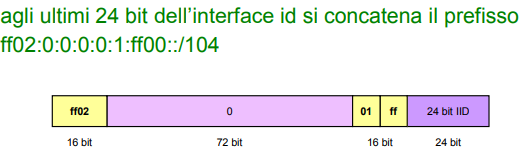
\includegraphics[width=14cm, height=3cm]{immagine_2025-01-02_122903684.png} % Percorso dell'immagine
   % \caption{Datagram Header} % Didascalia per l'immagine
    \label{fig:immagine} % Etichetta per riferimento
\end{figure}
\noindent
Per ottenere un indirizzo MAC di un sistema il nodo calcola l'indirizzo multicast solicited-node corrispondente all'indirizzo IPv6 del destinatario. Il nodo invia a questo indirizzo un pacchetto ICMPv6 di \textbf{neighbor solicitation} specificando l'indirizzo IPv6 del destinatario nel campo dati. Il destinatario, se presente, risponde con un pacchetto unicast di \textbf{neighbor advertisement}. Il suo indirizzo MAC è specificato nella parte dati del pacchetto, viene memorizzato nella neighbor cache. \textbf{Solicited node} viene utilizzato perchè, mentre un pacchetto broadcast è considerato da tutte le schede della LAN come ad esse destinato, un pacchetto multicast è considerato come ad esse destinato dalle sole schede di quel gruppo multicast. Visto che l'indirizzo solicited node contiene gli ultimi bit dell'indirizzo è probabile che venga processato da poche schede.
\begin{figure}[H] % 'h' per indicare di posizionare la figura qui
    \centering % Centra l'intera figura
    % Immagine di sinistra
    \begin{subfigure}[t]{0.45\textwidth} % Sottotitolo di dimensione 45% della larghezza
        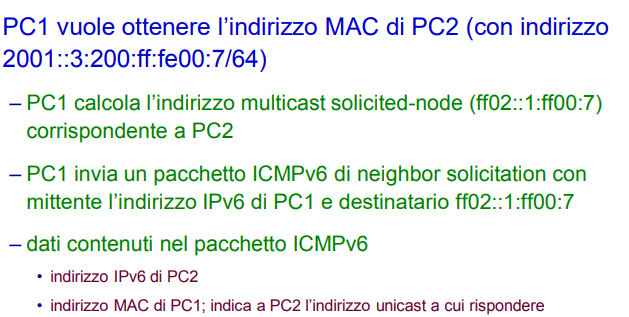
\includegraphics[width=\linewidth]{immagine_2025-01-02_125125051.png} % Percorso dell'immagine
       % \caption{Arrivo in precedenza dei processi più piccoli} % Didascalia per la prima immagine
        \label{fig:sinistra} % Etichetta per riferimento
    \end{subfigure}
    \hspace{0.05\textwidth} % Spazio orizzontale tra le immagini
    % Immagine di destra
    \begin{subfigure}[t]{0.45\textwidth} % Sottotitolo di dimensione 45% della larghezza
        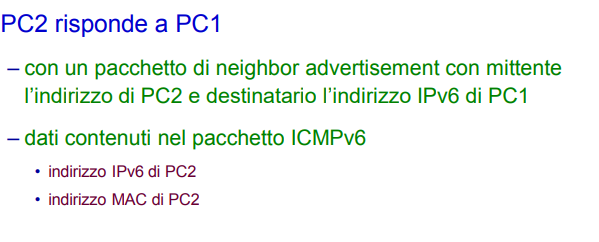
\includegraphics[width=\linewidth]{immagine_2025-01-02_125208592.png} % Percorso dell'immagine
       % \caption{Arrivo in precedenza del processo più grande} % Didascalia per la seconda immagine
        \label{fig:destra} % Etichetta per riferimento
    \end{subfigure}
   % \caption{SJF/Shortest Job First} % Didascalia generale per la figura
    \label{fig:due_immagini} % Etichetta generale per riferimento
\end{figure}
\noindent
\section{Lo strato di Trasporto}
Le primitive per l'instaurazione e per il rilascio di connessioni devono essere realizzate in modo affidabile. Il problema è più facile da risolvere per l'instaurazione di una connessione che per il rilascio.
\subsection{Instaurazione di connessioni}
I pacchetti scambiati nell'ambito di una connessione sono \textbf{numerati}, da entrambe le parti, in modo sequenziale (Così da poter riscontrare esplicitamente l'avvenuta ricezione di uno o più pacchetti con degli ACK). La numerazione dei pacchetti inizia da numeri scelti a piacere dalle due parti. L'instaurazione  è basata sulla scelta e sul relativo riscontro dei \textbf{numeri iniziali} di sequenza utilizzati per la numerazione dei pacchetti (\textbf{Metodo Three-way handshake}).
\begin{figure}[H]
    \centering
    \begin{minipage}{0.55\textwidth} % Imposta la larghezza della colonna sinistra
        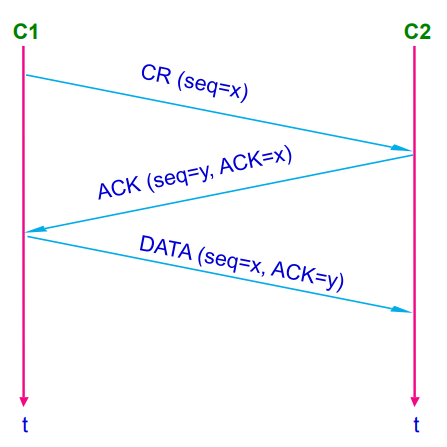
\includegraphics[width=8cm,height=6cm]{immagine_2025-01-03_105715416.png}
        %\caption{Routing by network address} % Opzionale
        \label{fig:immagine}
    \end{minipage}%
    \hfill
    \begin{minipage}{0.45\textwidth} % Imposta la larghezza della colonna destra
    \textbf{Metodo Three-way handshake} (Calcolatori C1 e C2):\\
    C1 sceglie il numero di sequenza iniziale x per i propri pacchetti\\
    C1 invia una Connection Request (CR) con x a C2\\
    C2 riceve la Connection Request con x\\
    C2 sceglie il proprio numero di sequenza iniziale y\\
    C2 invia una Connection Accepted riscontrando (ACK) x e proponendo il proprio numero iniziale y a C1\\
    C1 riscontra (ACK) y a C2
    \end{minipage}
\end{figure}
\noindent
Usare numeri diversi per ogni connessione consente di distinguere pacchetti che, pur scambiati dalla stessa coppia di interlocutori, magari in tempi diversi, appartengono a connessioni diverse.
\subsection{Rilascio di connessioni}
Il rilascio di connessioni è più difficile di quanto si possa immaginare. Per esempio: supponiamo di rilasciare la connessione come si termina una telefonata, ad un certo punto l'interlocutore C1 rilascia unilateralmente la connessione, se C2 aveva nel frattempo inviato dei dati c'è il rischio che essi arrivino a C1 dopo che C1 ha "attaccato il telefono" (smesso di ascoltare). Una possibile soluzione è il rilascio simmetrico: ogni direzione è rilasciata in modo indipendente dall'altra, quando un interlocutore ha rilasciato continua comunque a ricevere dati eventualmente provenienti dall'altro lato. In che istante la connessione può dirsi definitivamente rilasciata?
\begin{figure}[H]
    \centering
    \begin{minipage}{0.55\textwidth} % Imposta la larghezza della colonna sinistra
        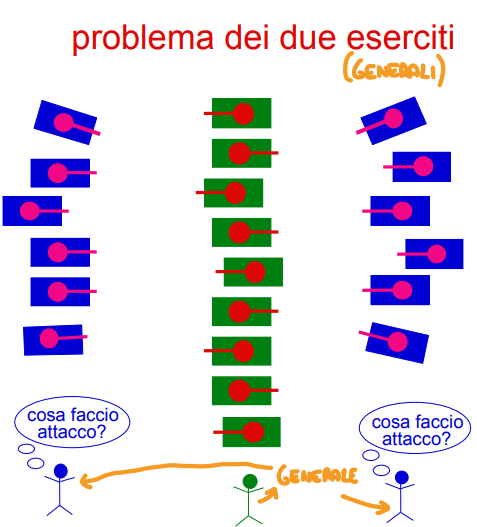
\includegraphics[width=8cm,height=6cm]{immagine_2025-01-03_110904065.png}
        %\caption{Routing by network address} % Opzionale
        \label{fig:immagine}
    \end{minipage}%
    \hfill
    \begin{minipage}{0.45\textwidth} % Imposta la larghezza della colonna destra
    Se i blu attaccassero contemporaneamente vincerebbero perchè numericamente in vantaggio, se i generali blu attaccassero uno alla volta perderebbero (svantaggio numerico). I Blue vogliono trovare quindi un modo per sincronizzarsi e attaccare contemporaneamente. L'emissario acquisisce un informazione ("Attacchiamo alle 12!"), quest'ultimo deve passare attraverso al campo verde e andare dal comandante blu. Il problema è che non si sa se l'emissario è riuscito a comunicare e quindi se non fosse arrivato i blu attaccherebbero in svantaggio. Allora l'altra parte di esercito blu manda un altro emissario per confermare l'attacco. Nuovamente non avverrà l'attacco, perchè l'altro esercito blu non sa se è arrivata la conferma. L'ultimo a spedire i riscontri non saprà mai se l'emissario sarà arrivato. La metafora è che i verdi sono internet, e che non siamo certi del fatto che quando mandiamo un pacchetto arrivi dall'altra parte.
    \end{minipage}
\end{figure}
\noindent
\subsection{TCP (Transmission Control Protocol)}
\textbf{TCP} è un servizio di trasmissione dati affidabile bidirezionale contemporaneo (full-duplex) punto-punto (host-to-host, end-to-end) (multicast e broadcast non sono supportati). \textbf{TCP} è il primo tra i protocolli studiati fino ad ora nella Internet Protocol Suite a garantire l'affidabilità del servizio di trasmissione. Al livello 3, a causa del traffico eccessivo o di errori di vario genere, i pacchetti possono andare perduti o essere consegnati nell'ordine sbagliato. \textbf{TCP} identifica questi problemi, richiede la ritrasmissione dei dati perduti e riordina i pacchetti ricevuti fuori ordine. \textbf{TCP} fa uso sitematico di riscontri (\textbf{Acknowledgement - ACK}).\\
Il servizio offerto da TCP è \textbf{connesso} e la connessione avviene fra due processi, identificati dall'\textbf{indirizzo IP} e da un numero di \textbf{port} da entrambe le parti. Una volta che la connessione è stabilita, il processo utente manda i dati allo strato \textbf{TCP} che li invia correttamente allo strato \textbf{TCP} del ricevente, che li offre a sua volta al processo destinazione. L'implementazione della connessione fa in modo che i processi utente vedano un canale di comunicazione privato, permettendo una programmazione a livello utente in cui la rete è \textbf{trasparente}.
\subsubsection{Port}
TCP specifica come distinguere più destinazioni (processi) su una stessa macchina. Ai processi che interagiscono con altri processi usando TCP viene attribuito un numero di \textbf{port}. I port sono i TCP SAP (Service Access Point). Un numero di port ha 2 byte. I port $<$ 1024 sono riservati per servizi standard.
\subsubsection{Pacchetti e Byte}
La t-pdu (pacchetto) TCP si chiama \textbf{segment}. \textbf{Segment} = header + dati (opzionali). TCP non numera i pacchetti ma i byte; ogni byte spedito ha un numero di sequenza a 32 bit. I numeri di sequenza sono usati anche per gli ACK. I segment vengono usati principalmente per: instaurare connessioni, spedire dati, spedire acknowledgement (ACK), chiudere connesioni.
\begin{figure}[H] % Usa 'H' per forzare la posizione qui
    \centering % Centra l'immagine
    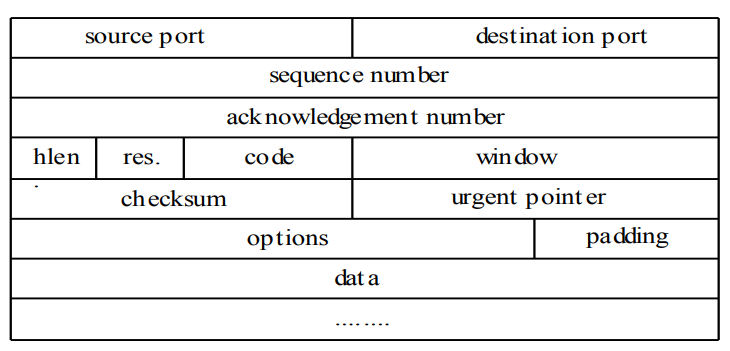
\includegraphics[width=12cm, height=5cm]{immagine_2025-01-03_113141334.png} % Percorso dell'immagine
   % \caption{Datagram Header} % Didascalia per l'immagine
    \label{fig:immagine} % Etichetta per riferimento
\end{figure}
\noindent
Il \textbf{sequence number} stabilisce la posizione del pacchetto dati nel flusso di informazioni del mittente, questi infatti trasferisce un flusso di dati generando un certo numero di pacchetti da inviare attraverso la rete.\\
L'\textbf{acknowledgement (ACK) number} viene utilizzato per riscontrare i byte ricevuti correttamente (significato: prossimo byte atteso).\\
Il \textbf{sequence number} si riferisce al flusso che va nella stessa direzione del segment mentre \textbf{ACK number} si riferisce al flusso che va in direzione opposta al segment.
\begin{figure}[H]
    \centering
    \begin{minipage}{0.55\textwidth} % Imposta la larghezza della colonna sinistra
        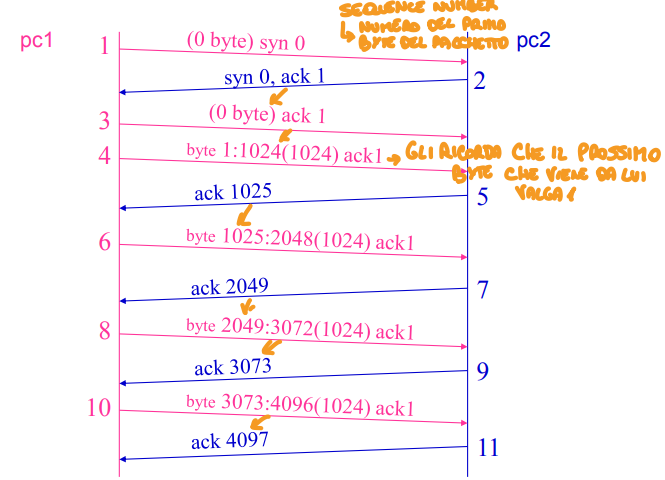
\includegraphics[width=10cm,height=6cm]{immagine_2025-01-03_113732604.png}
        %\caption{Routing by network address} % Opzionale
        \label{fig:immagine}
    \end{minipage}%
    \hfill
    \begin{minipage}{0.45\textwidth} % Imposta la larghezza della colonna destra
    \textbf{PC1} manda un byte di sincronizzazione. \textbf{PC2} risponde al byte di sincronizzazione riinviandolo indietro insieme ad un ACK (che dice una cosa del tipo "Hey mi aspetto che il prossimo byte sia 1". Successivamente viene inviato un nuovo ACK e inizia la trasmissione.
    \end{minipage}
\end{figure}
\noindent
\textbf{Hlen}: numero di parole di 32 bit dell'intestazione.\\
\textbf{Code}: determina il tipo di messaggio contenuto nel segmento - bit più importanti:
\textbf{ACK} quando è a 1 il riscontro è valido. \textbf{SYN (Synchronize sequence numbers)} e \textbf{FIN} questo è un pacchetto di richiesta di fine di una connessione.\\
\textbf{Urgent Pointer}: consente di stabilire dove si trovino eventuali dati urgenti presenti nel segment.\\
\textbf{Checksum}: interessa l'intero segment + indirizzi IP + protocol.\\
\textbf{Opzioni}: la più utilizzata specifica la massima ampiezza del campo dati. Negoziazione durante l'instaurazione della connessione (Le macchine comunicano per le MTU).\\
Per ogni connessione, TCP ha un \textbf{buffer} (memoria disponibile, gestita come una coda) \textbf{di trasmissione} e un \textbf{buffer di ricezione}. L'effetto di una primitiva \textbf{send} quello di inserire i dati da spedire nel buffer di trasmissione. TCP li spedirà attraverso la rete appena lo riterrà opportuno. L'effetto di una primitiva \textbf{receive} è quello di prelevare dati, già ricevuti da TCP, dal buffer di trasmissione. TCP, a questo punto, li cancella dal buffer di ricezione.\\
\textbf{Window} specifica la ampiezza corrente della \textbf{finestra di controllo di flusso}, stabilisce quanti byte il ricevente è in grado di ricevere dopo l'ultimo riscontrato (spazio disponibile nel buffer di ricezione). Limita i byte che possono essere inviati dall'interlocutore.\\
Quindi per il \textbf{rilascio di una connessione}:\\
Per rilasciare la connessione una delle due parti manda un segment con \textbf{FIN=1}; non ha più dati da trasmettere. Quando la parte che ha mandato \textbf{FIN=1} riceve in riscontro un \textbf{ACK} considera chiuso il suo flusso. I dati possono continuare a fluire in direzione opposta. La connessione è rilasciata quando entrambi i flussi sono chiusi. Il rilascio normale richiede 4 segment. Il primo \textbf{ACK} ed il secondo \textbf{FIN} possono essere nello stesso segment. Uso di timeout per il problema dei due eserciti; timeout = 2 * tempo di vita stimato di un pacchetto.
\begin{figure}[H] % Usa 'H' per forzare la posizione qui
    \centering % Centra l'immagine
    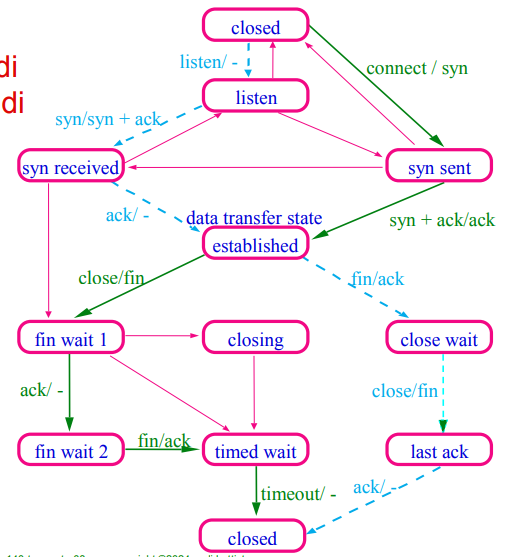
\includegraphics[width=9cm, height=6cm]{immagine_2025-01-03_121504240.png} % Percorso dell'immagine
   % \caption{Datagram Header} % Didascalia per l'immagine
    \label{fig:immagine} % Etichetta per riferimento
\end{figure}
\noindent
Lo stato \textbf{established} corrisponde a molti più stati specifici, sia in ricezione (riscontro dei pacchetti ricevuti correttamente, gestione della finestra di controllo di flusso) che in spedizione (scelte nella spedizione dei pacchetti, per sfruttare al massimo la banda e per contribuire al controllo delle congestioni nella rete, spedizione di copie dei pacchetti di cui non si è ottenuto un ack).
\subsection{UDP (User Datagram Protocol)}
\textbf{UDP} fornisce un servizio di trasmissione non connesso e non affidabile. Il mittente non ha informazioni (non riceve riscontri ACK) sull'esito effettivo della ricezione. Viene utilizzato da servizi nei quali: non è importante che un pacchetto sia riscontrato (si preferisce l'efficienza rispetto all'affidabilità), oppure si preferisce gestire il meccanismo riscontri a livello applicativo. L'header è diviso in 4 campi di 16 bit che specificano il port da cui viene inviato il messaggio, il port destinazione, la lunghezza datagram ed il checksum. I port UDP sono analoghi ai port TCP.
\section{DNS (Domain Name System)}
Esiste un meccanismo che permette di denotare un'interfaccia di rete specificandone il nome (più facile da ricordare), e che si occupa della traduzione del nome in un indirizzo IP (mapping). L'insieme dei nomi ammissibili è detto \textbf{namespace}. I nomi sono sequenze di caratteri separate da punti. I nomi che hanno un suffisso comune possono essere rappresentati con un \textbf{albero}.
\subsection{Gerarchia del namespace}
Il livello più alto (\textbf{top level}) (parte più a destra dell'indirizzo) della gerarchia partiziona lo spazio dei nomi e delega la gestione dei nomi delle diverse partizioni ad autorità locali. L'autorità top level non deve occuparsi di questioni interne alle partizioni. La gerarchia viene definita non in base alla collocazione fisica degli host nella rete, ma in accordo con la struttura dell'organizzazione a cui appartengono. 
\begin{figure}[H]
    \centering
    \begin{minipage}{0.55\textwidth} % Imposta la larghezza della colonna sinistra
        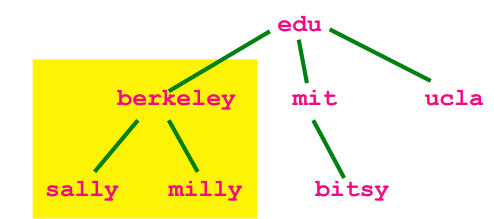
\includegraphics[width=8cm,height=4cm]{immagine_2025-01-03_125632008.png}
        %\caption{Routing by network address} % Opzionale
        \label{fig:immagine}
    \end{minipage}%
    \hfill
    \begin{minipage}{0.45\textwidth} % Imposta la larghezza della colonna destra
    Un \textbf{dominio} è un sottoalbero del namespace. Il nome del dominio è il nome della radice del sottoalbero. Es. berkeley.edu. Le foglie dell'albero rappresentano host (sono cioè associate a indirizzi IP); anche i nodi intermedi possono rappresentare host. Anche un singolo host è un dominio.
    \end{minipage}
\end{figure}
\noindent
Per generalità, si assue che tutti i domini \textbf{top-level} siano figli di un unico dominio radice, cui corrisponde la stringa vuota (""). L'organizzazione dei nomi di Internet è detta \textbf{Domain Name System (DNS)}. I sistemi che realizzano i mapping tra nomi ed indirizzi sono detti \textbf{name server (ns)}. Alcuni name server hanno la delega per una porzione del namespacce. I name server possono dialogare tra loro.\\
Un name server ha informazioni complete su una parte del namespace detto \textbf{zona}; quel name server è l'\textbf{autorità} per quella \textbf{zona}.
\begin{figure}[H] % Usa 'H' per forzare la posizione qui
    \centering % Centra l'immagine
    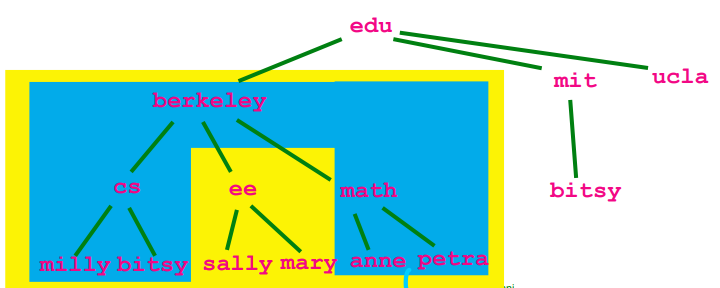
\includegraphics[width=8cm, height=4cm]{immagine_2025-01-03_130338657.png} % Percorso dell'immagine
   % \caption{Datagram Header} % Didascalia per l'immagine
    \label{fig:immagine} % Etichetta per riferimento
\end{figure}
\noindent
I concetti di \textbf{dominio (in giallo)} e \textbf{zona (in blu)} sono differenti. Un name server può essere l'autorità per varie zone. Alla stessa zona possono essere associati vari name server autorità. Relativamente a una zona i name server possono essere: \textbf{Primary} ha, nei suoi file di configurazione, la versione corretta e aggiornata delle informazioni di mapping della zona, \textbf{Secondary} richiede periodicamente al primary una copia aggiornata delle informazioni di mapping della zona. Un name server può essere contemporaneamente primary per certe zone e secondary per altre.
\subsection{Resolver e risoluzione}
I client che usano i name server si chiamano \textbf{resolver}. I resolver sono a bordo degli host e sanno: interrogare un name server, interpretare le risposte, inviare le informazioni ricavate ai programmi che li utilizzano. Quando un resolver chiede informazioni ad un name server, se il name server le ha le fornisce direttamente. Se il name server non le ha, esso si rivolge al name server autorità per la radice dello spazio dei nomi. Il name server autorità per la radice dello spazio dei nomi a sua volta indica al name server un name server più specifico. Il name server alla radice (in realtà ce ne sono vari) è molto sotto pressione ed ha migliaia di query ogni secondo.
\begin{figure}[H]
    \centering
    \begin{minipage}{0.55\textwidth} % Imposta la larghezza della colonna sinistra
        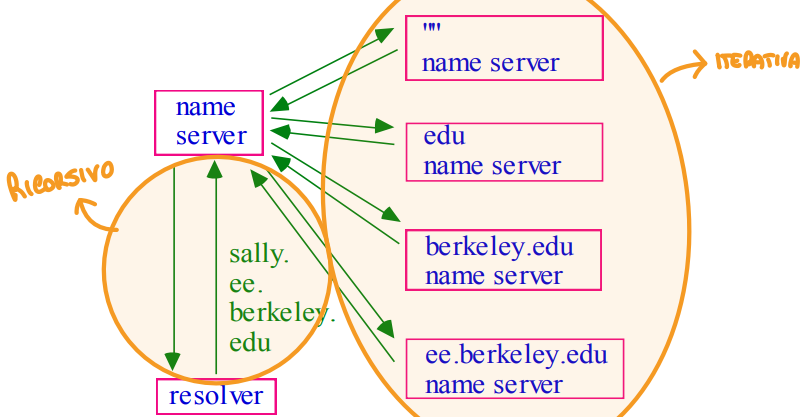
\includegraphics[width=9cm,height=4cm]{immagine_2025-01-03_134938122.png}
        %\caption{Routing by network address} % Opzionale
        \label{fig:immagine}
    \end{minipage}%
    \hfill
    \begin{minipage}{0.45\textwidth} % Imposta la larghezza della colonna destra
    La risoluzione può essere \textbf{ricorsiva} o \textbf{iterativa}. \textbf{Ricorsiva}: il client chiede a quale indirizzo corrisponda il nome \textbf{n} e pretende come risultato l'indirizzo; se il server non possiede l'indirizzo di \textbf{n} è suo compito contattare altri server per ottenerlo. \textbf{Iterativa}: il client chiede a quale indirizzo corrisponda il nome \textbf{n} e, in caso il server non lo abbia, si accontenta di un'indicazione di un altro server a cui rivolgersi.
    \end{minipage}
\end{figure}
\noindent
Durante ogni query un name server \textbf{apprende} informazioni sui nomi e sui server che svolgono il ruolo di autorità per le varie zone. Le informazioni apprese sono memorizzate in una \textbf{cache}. Alcuni server memorizzano anche informazioni negative. Anche le applicazioni hanno una \textbf{cache DNS}. Ovviamente è necessario definire il TTL delle informazioni in cache. \\
Alcuni ns non sono autorità per nessuna zona e sono solo a disposizione dei client. Normalmente ogni Internet Service Provider (Tim...) ne mette a disposizione uno per i propri utenti. Talvolta sono chiamati \textbf{Local name server} o \textbf{Caching name server} o \textbf{Recursive name server}.
\subsection{Resource record}
Le informazioni DNS sono memorizzate in \textbf{resource record}; ogni dominio è associato a uno o più \textbf{resource record}. I record contengono gli indirizzi IP, ma anche altre informazioni. Quando un resolver fa una query relativa a un nome ottiene come risposta i record associati a quel nome.
\begin{figure}[H] % Usa 'H' per forzare la posizione qui
    \centering % Centra l'immagine
    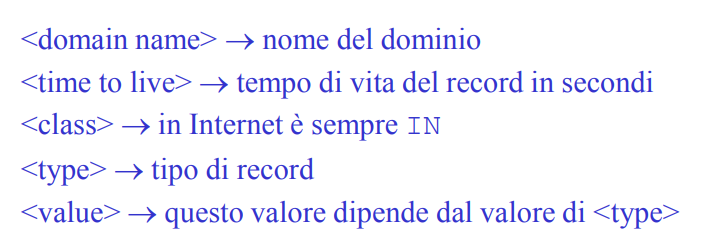
\includegraphics[width=10cm, height=4cm]{immagine_2025-01-03_140220584.png} % Percorso dell'immagine
   % \caption{Datagram Header} % Didascalia per l'immagine
    \label{fig:immagine} % Etichetta per riferimento
\end{figure}
\noindent
Ci sono vari type i principali sono: \textbf{SOA} contiene informazioni amministrative sulla zona, \textbf{A} indirizzo IPv4 di un host, \textbf{MX} specifica il nome dell'host che accetta le mail indirizzate al dominio del record, \textbf{NS} name server per una zona, \textbf{AAAA} indirizzo IPv6 di un host e \textbf{CNAME} canonical name; il nome corrisponde a un altro nome (alias).
\begin{figure}[H] % 'h' per indicare di posizionare la figura qui
    \centering % Centra l'intera figura
    % Immagine di sinistra
    \begin{subfigure}[t]{0.45\textwidth} % Sottotitolo di dimensione 45% della larghezza
        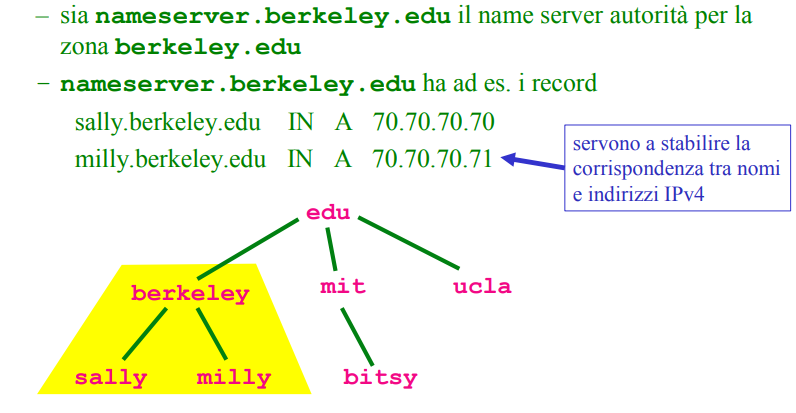
\includegraphics[width=10cm, height=6cm]{Screenshot 2025-01-03 140707.png} % Percorso dell'immagine
       % \caption{Arrivo in precedenza dei processi più piccoli} % Didascalia per la prima immagine
        \label{fig:sinistra} % Etichetta per riferimento
    \end{subfigure}
    \hspace{0.05\textwidth} % Spazio orizzontale tra le immagini
    % Immagine di destra
    \begin{subfigure}[t]{0.45\textwidth} % Sottotitolo di dimensione 45% della larghezza
        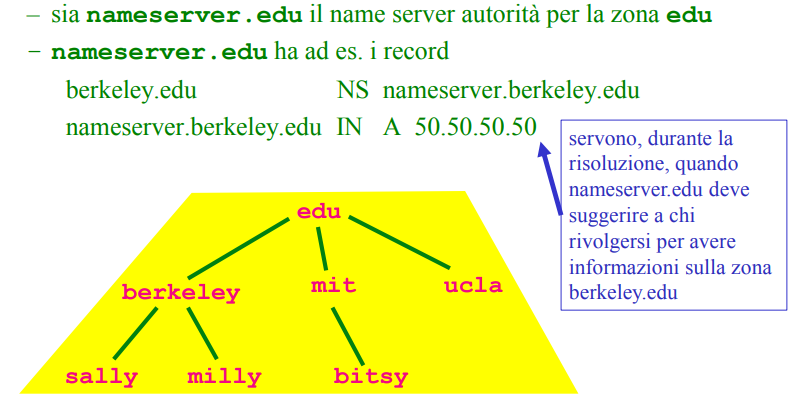
\includegraphics[width=10cm, height=6cm]{Screenshot 2025-01-03 140721.png} % Percorso dell'immagine
       % \caption{Arrivo in precedenza del processo più grande} % Didascalia per la seconda immagine
        \label{fig:destra} % Etichetta per riferimento
    \end{subfigure}
   % \caption{SJF/Shortest Job First} % Didascalia generale per la figura
    \label{fig:due_immagini} % Etichetta generale per riferimento
\end{figure}
\noindent
Il record di tipo A sembra al posto sbagliato dovrebbe essere su nameserver.berkeley.edu è qui per permettere la risoluzione. Si chiama \textbf{glue record}. \\
Per quanto riguarda il formato dei messaggi DNS ce ne sono di due tipi: richieste e risposte. Tra i campi dell'header: \textbf{QR} indica se il messaggio è una domanda o una risposta, \textbf{RD} recursion desired, indica se la query è ricorsiva. Tra i campi della question section: \textbf{NAME} nome della risorsa richiesta, \textbf{TYPE} tipo del resource record richiesto.\\
Normalmente i messaggi DNS viaggiano, a livello 4, su \textbf{UDP}. Questo perchè i pacchetti di richiesta e risposta sono piccoli, con TCP dovrei utilizzare tutti i suoi strumenti e aumentarne il tempo. I client si rivolgono alla well known port UDP 53. La richiesta viaggia in un singolo pacchetto UDP, la risposta viaggia in un singolo pacchetto UDP. Per dialoghi richiesta risposta che richiedono risposte di grandi dimensioni si può usare TCP. \\
Comando molto utile per vedere il comportamento DNS è \textbf{dig}. Si può utilizzare dig www.nome.it, si può aggiungere \textbf{+norecurse} per forzare il sistema a una query iterativa e si può mettere \textbf{+trace} per simulare le richieste di un ns.

\section{HTML (HyperText Markup Language)}
HTML è un linguaggio per la codifica di \textbf{ipertesti} (può contenere al suo interno dei riferimenti ad altri ipertesti) tramite \textbf{marcatori} (codice che segnala l'inizio (o la fine) di una primitiva di formattazione del testo).
\subsection{Ipertesti e marcatori}
Un ipertesto è quindi un testo con delle caratteristiche speciali. Una pagina contiene solo le informazioni essenziali, eventuali subordinate del discorso vengono distribuite su altre pagine, l'utente \textbf{naviga} tra le varie pagine a suo piacimento. Caratteristiche degli ipertesti:
\textbf{Concisione}: il contenuto di una singola pagina può essere ridotto all'essenziale, perchè la descrizione di eventuali dettagli aggiuntivi può essere rinviata ad altre pagine. \textbf{Completezza}: l'informazione complessiva, distribuita nelle varie pagine, può spingersi fino ad un livello di dettaglio arbitrario. \textbf{Condivisione}: i dati non vengono replicati ma condivisi, evitando quindi ridondanze. L'ipertesto costituito dall'insieme di tutte le pagine presenti su internet viene denominato \textbf{World Wide Web}. Occorre distinguere tra: \textbf{Internet}: "la rete delle reti" l'insieme di tutte le lan e delle loro connessioni, si riferisce alla struttura fisica, ma, per estensione, spesso allude a tutti i servizi disponibili in questo ambiente distribuito. \textbf{WWW} è la rete logica costituita dalle pagine web e dai loro hyperlink, la consultazione delle pagine web è solo uno dei servizi disponibili su internet. Si utilizza il \textbf{linguaggio dei marcatori} quando dobbiamo codificare un informazione la quale: può essere strutturata in maniera sequenziale, i cui attributi hanno delle proprietà locali (esempio testo in neretto). \textbf{Marcatura fisica} descrive dettagliatamente come apparirà il testo formattato. \textbf{Marcatura logica o semantica} descrive il significato strutturale (la funzione, il ruolo) degli oggetti da formattare. 
\subsection{Struttura HTML}
Una pagina HTML viene mostrata a schermo a seconda del \textbf{browser}, che decide come ogni singolo elemento posssa essere reso visivamente. Tutti i marcatori iniziano con $<$ e finiscono con $>$, i marcatori di fine formazione iniziano con uno slash dopo la parentesi angolata aperta. Alcuni marcatori ammettono attributi e i commenti hanno una forma del tipo $<!-- commento-->$. Dato che le parentesi angolari vengono utilizzate per i marcatori, quest'ultime non sono disponibili come caratteri testuali per questo motivo sono stati definiti i \textbf{caratteri speciali} i quali iniziano con \textbf{\&} e finiscono con \textbf{;}. Nella parte iniziale della pagina HTML è presente il comando \textbf{$<head>$} nel quale vengono inserite informazioni relative all'intera pagina HTML. Successivamente vi è il comando \textbf{$<body>$} nel quale vi è la descrizione degli oggetti da visualizzare. Lo stesso body può contenere degli attributi.
\begin{figure}[H] % 'h' per indicare di posizionare la figura qui
    \centering % Centra l'intera figura
    % Immagine di sinistra
    \begin{subfigure}[t]{0.45\textwidth} % Sottotitolo di dimensione 45% della larghezza
        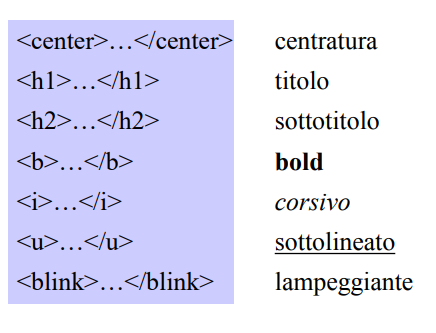
\includegraphics[width=7cm, height=5cm]{Screenshot 2025-01-04 114646.png} % Percorso dell'immagine
       % \caption{Arrivo in precedenza dei processi più piccoli} % Didascalia per la prima immagine
        \label{fig:sinistra} % Etichetta per riferimento
    \end{subfigure}
    \hspace{0.05\textwidth} % Spazio orizzontale tra le immagini
    % Immagine di destra
    \begin{subfigure}[t]{0.45\textwidth} % Sottotitolo di dimensione 45% della larghezza
        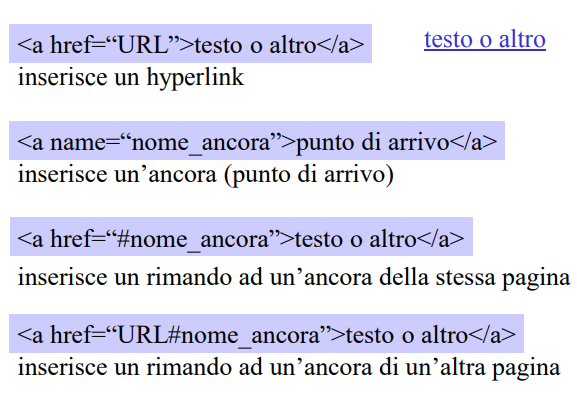
\includegraphics[width=7cm, height=5cm]{Screenshot 2025-01-04 114657.png} % Percorso dell'immagine
       % \caption{Arrivo in precedenza del processo più grande} % Didascalia per la seconda immagine
        \label{fig:destra} % Etichetta per riferimento
    \end{subfigure}
   % \caption{SJF/Shortest Job First} % Didascalia generale per la figura
    \label{fig:due_immagini} % Etichetta generale per riferimento
\end{figure}
\noindent
\begin{figure}[H] % 'h' per indicare di posizionare la figura qui
    \centering % Centra l'intera figura
    % Immagine di sinistra
    \begin{subfigure}[t]{0.45\textwidth} % Sottotitolo di dimensione 45% della larghezza
        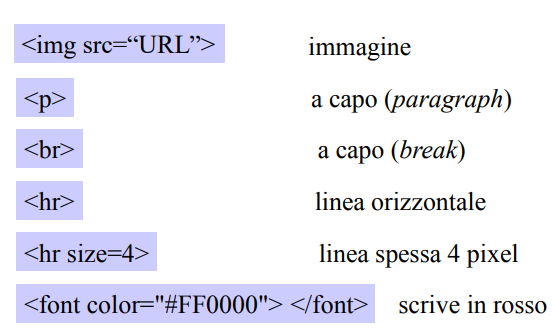
\includegraphics[width=7cm, height=5cm]{Screenshot 2025-01-04 114707.png} % Percorso dell'immagine
       % \caption{Arrivo in precedenza dei processi più piccoli} % Didascalia per la prima immagine
        \label{fig:sinistra} % Etichetta per riferimento
    \end{subfigure}
    \hspace{0.05\textwidth} % Spazio orizzontale tra le immagini
    % Immagine di destra
    \begin{subfigure}[t]{0.45\textwidth} % Sottotitolo di dimensione 45% della larghezza
        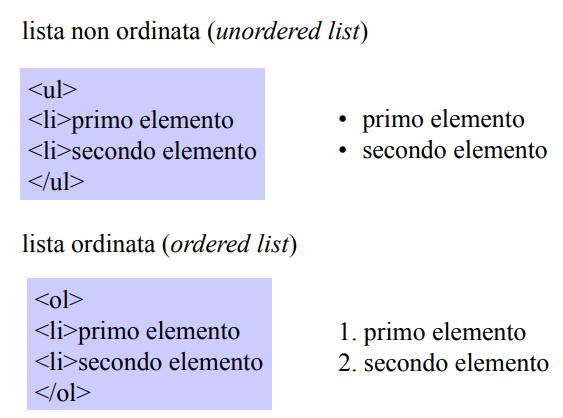
\includegraphics[width=7cm, height=5cm]{Screenshot 2025-01-04 114716.png} % Percorso dell'immagine
       % \caption{Arrivo in precedenza del processo più grande} % Didascalia per la seconda immagine
        \label{fig:destra} % Etichetta per riferimento
    \end{subfigure}
   % \caption{SJF/Shortest Job First} % Didascalia generale per la figura
    \label{fig:due_immagini} % Etichetta generale per riferimento
\end{figure}
\noindent
\begin{figure}[H] % 'h' per indicare di posizionare la figura qui
    \centering % Centra l'intera figura
    % Immagine di sinistra
    \begin{subfigure}[t]{0.45\textwidth} % Sottotitolo di dimensione 45% della larghezza
        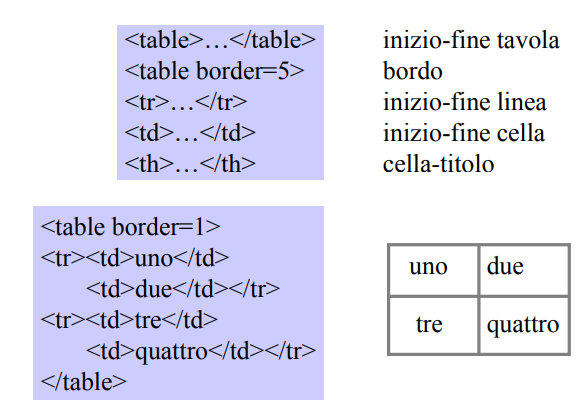
\includegraphics[width=7cm, height=5cm]{Screenshot 2025-01-04 114724.png} % Percorso dell'immagine
       % \caption{Arrivo in precedenza dei processi più piccoli} % Didascalia per la prima immagine
        \label{fig:sinistra} % Etichetta per riferimento
    \end{subfigure}
    \hspace{0.05\textwidth} % Spazio orizzontale tra le immagini
    % Immagine di destra
    \begin{subfigure}[t]{0.45\textwidth} % Sottotitolo di dimensione 45% della larghezza
        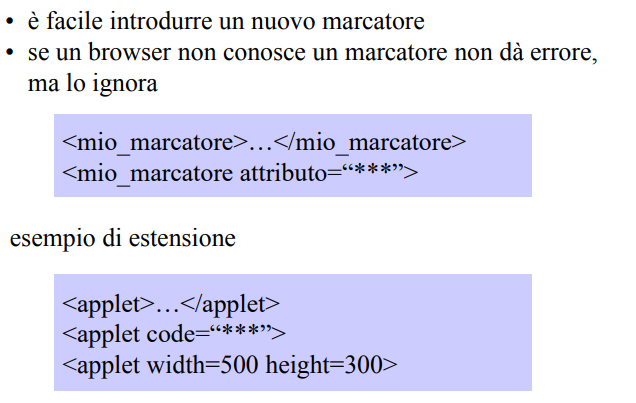
\includegraphics[width=7cm, height=5cm]{Screenshot 2025-01-04 114735.png} % Percorso dell'immagine
       % \caption{Arrivo in precedenza del processo più grande} % Didascalia per la seconda immagine
        \label{fig:destra} % Etichetta per riferimento
    \end{subfigure}
   % \caption{SJF/Shortest Job First} % Didascalia generale per la figura
    \label{fig:due_immagini} % Etichetta generale per riferimento
\end{figure}
\noindent
\section{URL e il protocollo HTTP}
\subsection{URL o URI (Uniform Resource Locator)}
Un \textbf{URL} è la rappresentazione testuale e compatta di una risorsa disponibile in internet.
\begin{figure}[H] % Usa 'H' per forzare la posizione qui
    \centering % Centra l'immagine
    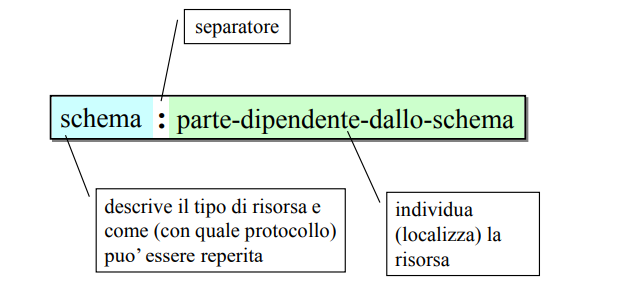
\includegraphics[width=10cm, height=3cm]{immagine_2025-01-06_110659576.png} % Percorso dell'immagine
   % \caption{Datagram Header} % Didascalia per l'immagine
    \label{fig:immagine} % Etichetta per riferimento
\end{figure}
\noindent
Della parte \textbf{schema} ne sono un esempio: telnet, ftp, http,... Per quando riguarda \textbf{la parte-dipendente-dallo-schema} solitamente si adotta la medesima sintassi. Sintassi che viene chiamata \textbf{C}ommon \textbf{I}nternet \textbf{S}cheme \textbf{S}yntax ("sintassi comune dello schema Internet")
\begin{figure}[H] % Usa 'H' per forzare la posizione qui
    \centering % Centra l'immagine
    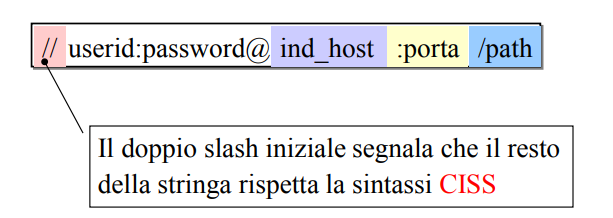
\includegraphics[width=10cm, height=3cm]{immagine_2025-01-06_111029863.png} % Percorso dell'immagine
   % \caption{Datagram Header} % Didascalia per l'immagine
    \label{fig:immagine} % Etichetta per riferimento
\end{figure}
\noindent
\textbf{userid:password@} è un campo che può mancare o essere parzialmente presente, \textbf{$ind\_host$} è l'indirizzo di una macchina: il suo numero IP o la sua stringa identificativa. \textbf{:porta} quando manca viene presa quella di default per lo schema in oggetto (es. http porta 80). \textbf{/path} indica un file all'interno del server.
\subsection{Il protocollo HTTP HyperText Transfer Protocol}
\begin{figure}[H] % Usa 'H' per forzare la posizione qui
    \centering % Centra l'immagine
    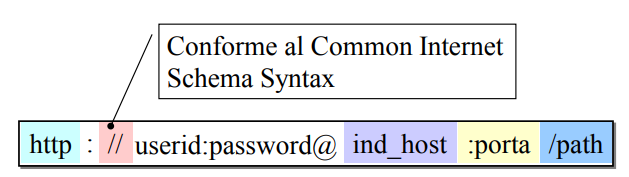
\includegraphics[width=10cm, height=2cm]{immagine_2025-01-06_111447005.png} % Percorso dell'immagine
   % \caption{Datagram Header} % Didascalia per l'immagine
    \label{fig:immagine} % Etichetta per riferimento
\end{figure}
\noindent
Quando un browser deve accedere ad una risorsa individuata da un URL estrae i campi \textbf{$ind\_host$} e \textbf{:porta} e li utilizza per aprire una connessione \textbf{tcp-ip} con il server. Se la porta non è specificata viene usata la porta di default per il protocollo http (porta 80). Il campo \textbf{userid:password@} viene utilizzato dal browser per gestire il colloquio eventuale con il server (richiesta di userid e password) senza coinvolgere l'utente. Il campo \textbf{/path} è un cammino nel file system del server. In coda può esserci: una stringa preceduta da \# (è un ancora, viene utilizzata dal client per posizionarsi sulla pagina html) o una stringa preceduta da ? (inviata al server).\\
Il protocollo HTTP è basato su un semplice schema richiesta risposta nel quale la richiesta è inviata da un client e la risposta è inviata da un server. Un colloquio client-server HTTP è una \textbf{sessione}.
\subsubsection{Sessione HTTP 1.0}
\begin{figure}[H] % 'h' per indicare di posizionare la figura qui
    \centering % Centra l'intera figura
    % Immagine di sinistra
    \begin{subfigure}[t]{0.45\textwidth} % Sottotitolo di dimensione 45% della larghezza
        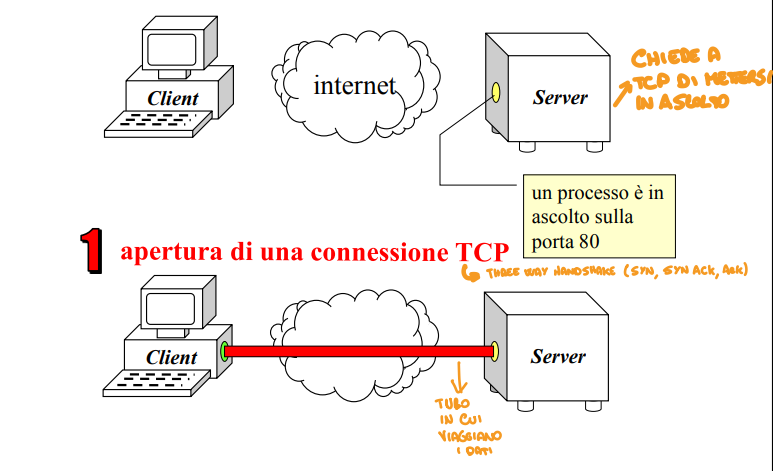
\includegraphics[width=9cm, height=5cm]{immagine_2025-01-06_112629519.png} % Percorso dell'immagine
       % \caption{Arrivo in precedenza dei processi più piccoli} % Didascalia per la prima immagine
        \label{fig:sinistra} % Etichetta per riferimento
    \end{subfigure}
    \hspace{0.05\textwidth} % Spazio orizzontale tra le immagini
    % Immagine di destra
    \begin{subfigure}[t]{0.45\textwidth} % Sottotitolo di dimensione 45% della larghezza
        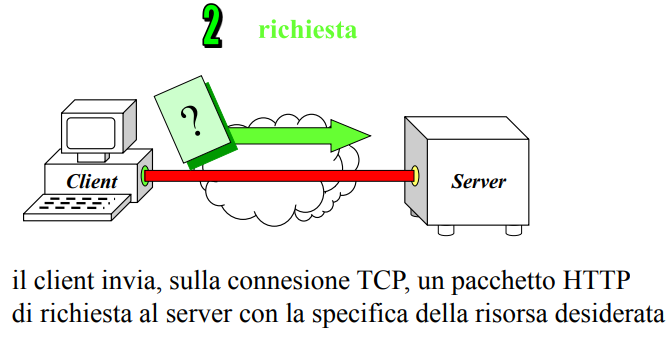
\includegraphics[width=9cm, height=5cm]{immagine_2025-01-06_112758935.png} % Percorso dell'immagine
       % \caption{Arrivo in precedenza del processo più grande} % Didascalia per la seconda immagine
        \label{fig:destra} % Etichetta per riferimento
    \end{subfigure}
   % \caption{SJF/Shortest Job First} % Didascalia generale per la figura
    \label{fig:due_immagini} % Etichetta generale per riferimento
\end{figure}
\begin{figure}[H] % 'h' per indicare di posizionare la figura qui
    \centering % Centra l'intera figura
    % Immagine di sinistra
    \begin{subfigure}[t]{0.45\textwidth} % Sottotitolo di dimensione 45% della larghezza
        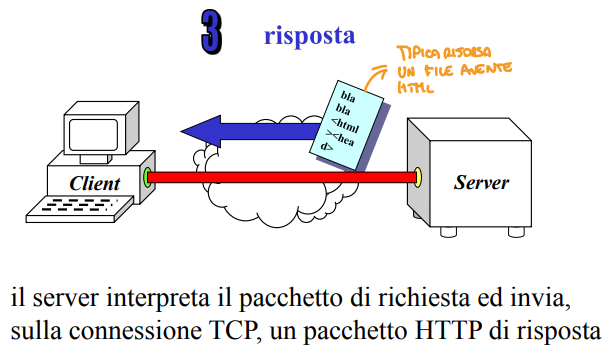
\includegraphics[width=9cm, height=5cm]{Screenshot 2025-01-06 112839.png} % Percorso dell'immagine
       % \caption{Arrivo in precedenza dei processi più piccoli} % Didascalia per la prima immagine
        \label{fig:sinistra} % Etichetta per riferimento
    \end{subfigure}
    \hspace{0.05\textwidth} % Spazio orizzontale tra le immagini
    % Immagine di destra
    \begin{subfigure}[t]{0.45\textwidth} % Sottotitolo di dimensione 45% della larghezza
        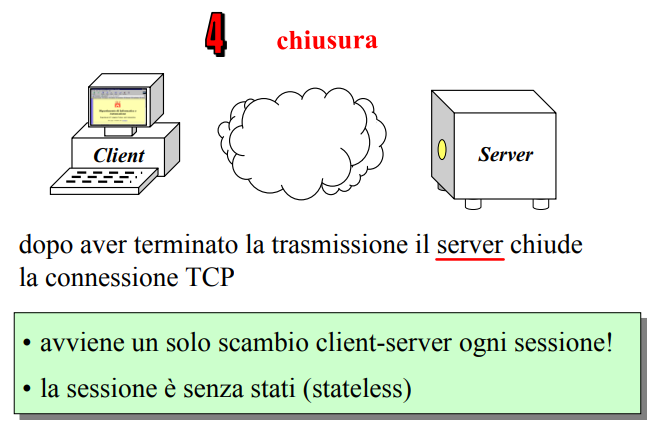
\includegraphics[width=9cm, height=5cm]{immagine_2025-01-06_112935334.png} % Percorso dell'immagine
       % \caption{Arrivo in precedenza del processo più grande} % Didascalia per la seconda immagine
        \label{fig:destra} % Etichetta per riferimento
    \end{subfigure}
   % \caption{SJF/Shortest Job First} % Didascalia generale per la figura
    \label{fig:due_immagini} % Etichetta generale per riferimento
\end{figure}
\noindent
\begin{figure}[H] % Usa 'H' per forzare la posizione qui
    \centering % Centra l'immagine
    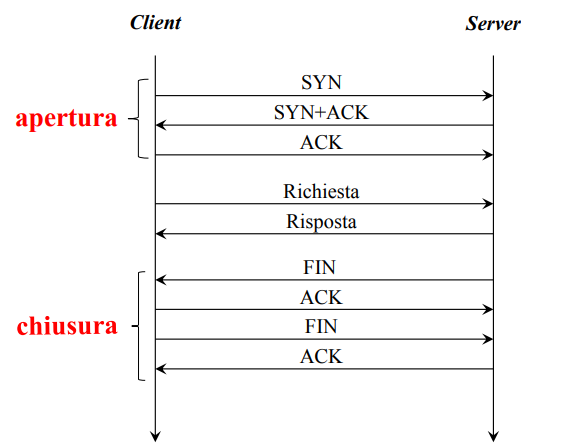
\includegraphics[width=10cm, height=5cm]{immagine_2025-01-06_113051481.png} % Percorso dell'immagine
   % \caption{Datagram Header} % Didascalia per l'immagine
    \label{fig:immagine} % Etichetta per riferimento
\end{figure}
\noindent
Per quanto riguarda i \textbf{pacchetti HTTP} ci sono due tipi di pacchetti: richiesta e risposta. Una \textbf{richiesta} HTTP si riferisce ad una risorsa, un metodo di \textbf{richiesta} HTTP specifica quale azione si voglia eseguire su tale risorsa. I principali metodi di richiesta HTTP sono: \textbf{GET} richiede la risorsa indicata, \textbf{POST} invia dati alla risorsa indicata, \textbf{HEAD} chiede informazioni sulla risorsa indicata, \textbf{PUT} ricopia i dati inviati sulla risorsa indicata, sostituendo il file presente, \textbf{DELETE} richiede la cancellazione di una risorsa, \textbf{OPTIONS} richiede di conoscere quali opzioni sono disponibili per il trasferimento della risorsa specificata.
\begin{figure}[H] % Usa 'H' per forzare la posizione qui
    \centering % Centra l'immagine
    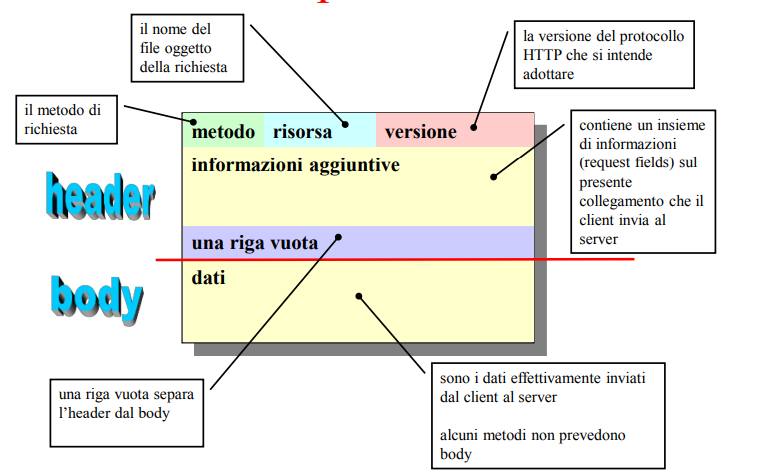
\includegraphics[width=11cm, height=7cm]{Screenshot 2025-01-06 113652.png} % Percorso dell'immagine
   % \caption{Datagram Header} % Didascalia per l'immagine
    \label{fig:immagine} % Etichetta per riferimento
\end{figure}
\noindent
Struttura di un pacchetto di \textbf{risposta}:
\begin{figure}[H] % Usa 'H' per forzare la posizione qui
    \centering % Centra l'immagine
    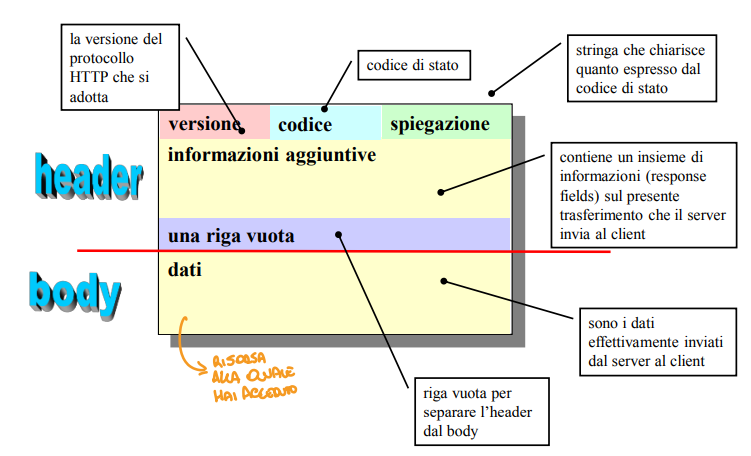
\includegraphics[width=11cm, height=6cm]{Screenshot 2025-01-06 113923.png} % Percorso dell'immagine
   % \caption{Datagram Header} % Didascalia per l'immagine
    \label{fig:immagine} % Etichetta per riferimento
\end{figure}
\noindent
Tra i codici di stato troviamo: \\
\textbf{Il server riesce a soddisfare la richiesta del client}:
\textbf{200} il pacchetto contiene ciò che è stato richiesto dal client, \textbf{201} è stata creata una nuova risorsa come richiesto, \textbf{202} è stata accettata la richiesta, ma la nuova risorsa non è ancora stata creata\\
\textbf{Azioni richieste per completare l'azione}: \textbf{301} la risorsa è disponibile ad un altro indirizzo, \textbf{304} la risorsa non è stata modificata.\\
\textbf{La richiesta è errata e non può essere soddisfatta}: \textbf{400} sintassi della richiesta non corretta, \textbf{401} autorizzazione richiesta, \textbf{403} risorsa esistente ma non disponibile, \textbf{404} risorsa non esistente, \textbf{405} metodo non permesso per la risorsa specificata, \textbf{414} nome della risorsa troppo lungo\\
\textbf{Non può essere soddisfatta una richiesta legittima}: \textbf{500} errore interno del server non meglio specificato, \textbf{501} funzionalità non implementata, \textbf{505} versione HTTP non supportata.\\
Tra i \textbf{request fields} invece troviamo \textbf{cookie} un cookie inviato dal server in precedenza (il server ha usato set-cookie), \textbf{host} il domain name del server e il numero di port TCP (opzionale se 80); utile per servire vari domini sullo stesso server.\\
Un \textbf{cookie} è un dato spedito dal server e memorizzato nel client (browser), viene re-inviato dal client al server ogni volta che il client accede a certe risorse (scope del cookie), viene usato per gestire una forma di 'stato' nelle sessioni HTTP, in questo modo il server ricorstruisce attività precedenti del client. Tra le applicazioni dei cookie troviamo: memorizzare gli oggetti selezionati da un cliente in un negozio online.
\subsubsection{Connessioni persistenti - HTTP 1.1}
Contrariamente a quanto specificato nel funzionamento di base (HTTP 1.0) è tipico (a partire da HTTP 1.1) che sulla stessa connessione TCP, un client possa effettuare più richieste consecutive ed ottenere le relative risposte. Il server ha comunque la possibilità di chiudere la connessione TCP quando lo ritiene opportuno. Tra TCP e HTTP viene usato un protocollo che ha l'obiettivo di rendere sicura la connessione (TLS - Transport Layer Security), infatti dopo il three-way-handshake le due parti devono scambiarsi le informazioni per il funzionamento del protocollo sicuro.
\begin{figure}[H] % Usa 'H' per forzare la posizione qui
    \centering % Centra l'immagine
    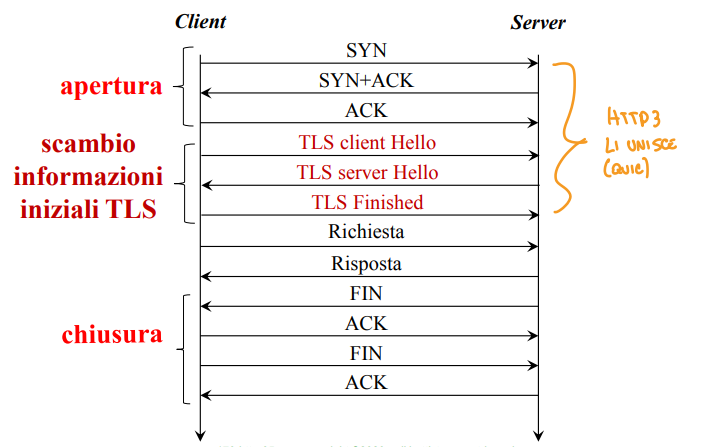
\includegraphics[width=8cm, height=4cm]{immagine_2025-01-06_120122764.png} % Percorso dell'immagine
   % \caption{Datagram Header} % Didascalia per l'immagine
    \label{fig:immagine} % Etichetta per riferimento
\end{figure}
\noindent
Se è possibile fare una sola richiesta per ogni connessione TCP allora, per ogni richiesta, ai 7 pacchetti di apertura-chiusura si sommano quelli per TLS e l'overhead per ciascuna richiesta diventa eccessivo. Quando si usa HTTP su TLS la porta di ascolto di default del server è 443. In HTTP 1.1 una nuova richiesta può essere inviata solo dopo aver ricevuto la risposta della richiesta precedente, in \textbf{HTTP/2} un browser può inviare varie richieste contemporanee sulla stessa connessione TCP (HTTP pipelining). \textbf{HTTP/3} utilizza un nuovo protocollo di trasporto chiamato \textbf{QUIC}. \textbf{QUIC} usa pacchetti UDP (è come se fosse un TCP personale) infatti QUIC è in User-space e quindi gli upgrade sul protocollo non sono legati agli upgrade del sistema operativo. In QUIC il three-way-handshake è mischiato con l'handshake di TLS.
\section{La posta elettronica (progettazione di un servizio di rete)}
\subsection{Progettazione di un servizio di rete}
\textbf{Fasi della progettazione di un servizio}:
\textbf{Analisi dei requisiti}: definizione delle caratteristiche del servizio
\textbf{Specifica delle primitive di servizio}: definizione dell'interfaccia al servizio.
\textbf{Definizione dell'architettura e delle operazioni}: definizione delle applicazioni coinvolte nella gestione del servizio, dei servizi ausiliari di rete necessari, degli ambienti di supporto, delle operazioni e dei flussi di informazione.
\textbf{Definizione dei protocolli}: per ogni tipologia di comunicazione definizione della struttura delle PDU (envelope e data), degli stati e delle procedure (regole d'uso) del protocollo. Nell'analisi dei requisiti si vanno a gestire messaggi in partenza e messaggi ricevuti e successivamente quali primitive di servizio usare per gestirli. Per quanto riguarda l'architettura, abbiamo visto più ipotesi:
\begin{figure}[H] % Usa 'H' per forzare la posizione qui
    \centering % Centra l'immagine
    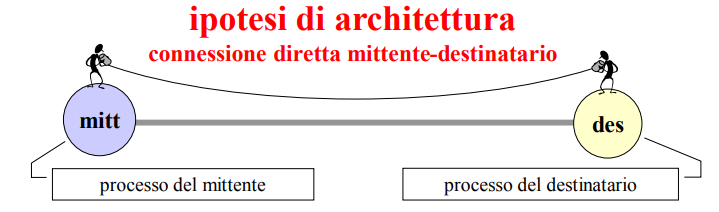
\includegraphics[width=11cm, height=2cm]{Screenshot 2025-01-06 123440.png} % Percorso dell'immagine
   % \caption{Datagram Header} % Didascalia per l'immagine
    \label{fig:immagine} % Etichetta per riferimento
\end{figure}
\noindent
Tra i \textbf{vantaggi} di questa prima ipotesi: semplicità di implementazione, recapito in tempo reale del messaggio, certezza della consegna. Tra gli \textbf{svantaggi}: il mittente non può spedire il messaggio se il destinatario non ha posto in esecuzione il suo processo, oppure ha spento il computer. Il mittente deve ricordare il nome della macchina del destinatario. Non è chiaro come si possa autenticare il destinatario.
\begin{figure}[H] % Usa 'H' per forzare la posizione qui
    \centering % Centra l'immagine
    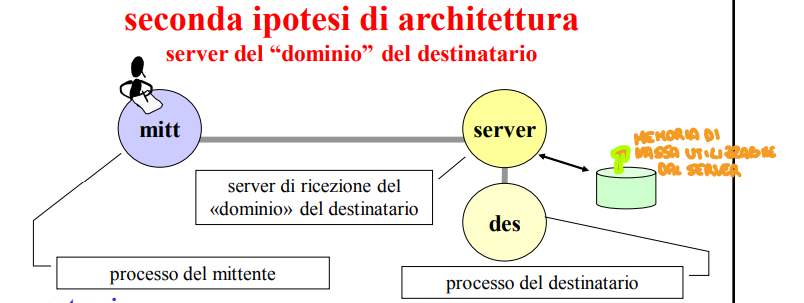
\includegraphics[width=11cm, height=3cm]{immagine_2025-01-06_124056279.png} % Percorso dell'immagine
   % \caption{Datagram Header} % Didascalia per l'immagine
    \label{fig:immagine} % Etichetta per riferimento
\end{figure}
\noindent
\textbf{Vantaggi}: i processi di invio e ricezione del messaggio sono disaccoppiati, il destinatario può essere autenticato dal server, il mittente deve ricordare solo il dominio del destinatario. \textbf{Svantaggi}: il server può essere guasto o impegnato, e il mittente può chiudere il suo programma prima che il messaggio sia recapitato.
\begin{figure}[H] % Usa 'H' per forzare la posizione qui
    \centering % Centra l'immagine
    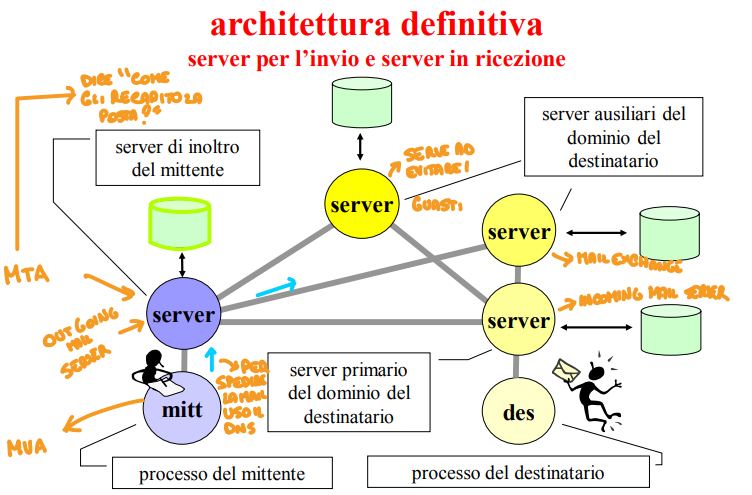
\includegraphics[width=11cm, height=6cm]{immagine_2025-01-06_124353569.png} % Percorso dell'immagine
   % \caption{Datagram Header} % Didascalia per l'immagine
    \label{fig:immagine} % Etichetta per riferimento
\end{figure}
\noindent
Un'indirizzo email è composto da due parti, separate dal simbolo @, la prima parte identifica un \textbf{utente}, la seconda parte è il nome di un \textbf{dominio}. In un servizio di posta elettronica sono coinvolte nel servizio due applicazioni: \textbf{MUA (Mail User Agent)} detto anche mailer, implementa un'interfaccia per l'utente, l'utente lo manda in esecuzione quando vuole accedere al servizio di posta elettronica (e lo può interrompere subito dopo aver usato le primitive che gli interessano). \textbf{MTA (Mail Transmission Agent)} è un'applicazione che fa da intermediaria nel processo di trasmissione del messaggio dalla sorgente fino alla destinazione. Il servizio è offerto in maniera il più possibile continuativa e stabile nel tempo. Ruolo dei server che ospitano un MTA: \textbf{Outgoing Mail Server} il computer il cui \textbf{MTA} è quello a cui fa diretto riferimento il \textbf{MUA} per l'inoltro della posta (server lanciatore). \textbf{Mail eXchanger} ogni dominio definisce nel DNS una lista di host (in ordine di priorità) che ospitano gli \textbf{MTA} che sono incaricati di ricevere posta per quel dominio (server ricevitore). \textbf{Incoming Mail Server} è il computer che ospita l'\textbf{MTA} da cui il \textbf{MUA} ritira la posta; generalmente coincide con il Mail eXchanger primario del dominio. \\
Ora il requisito che il MUA sia facilmente configurabile è soddisfatto: si richiede la sola specifica dei nomi dell'\textbf{outgoing mail server} e dell'\textbf{incoming mail server}. È necessario definire come ogni primitiva possa essere evasa tramite una successione di operazioni eseguite dalle applicazioni coinvolte. Es. tutte le primitive di \textbf{gestione dei messaggi in partenza e dei messaggi ricevuti} sono delegati al MUA.\\\\
\textbf{Spedizione di un messaggio}: il MUA trasmette il messaggio al suo Outgoing Mail Server, il Mail Server richiede (tramite il DNS) la lista dei Mail eXchanger del dominio destinazione (in ordine di priorità) e cerca di trasmettere il messaggio ad uno di essi; se fallisce con tutti, salva la mail nel suo file system e riprova ad inoltrarla ad intervalli di tempo regolari; se fallisce per tre giorni consecutivi
notifica al mittente il fallimento. un Mail eXchanger secondario cerca ad intervalli di tempo regolari di trasmettere il messaggio al Mail eXchanger primario.\\\\
Tra i \textbf{servizi ausiliari al servizio di posta elettronica}. DNS (Domain Name System): necessario all’Outgoing Mail Server per ottenere la lista e la priorità dei Mail eXchanger del dominio destinazione. File System Distribuito: se l’incoming mail server non coincide con il Mail eXchanger primario del dominio destinazione, l’incoming mail server deve poter accedere ai file delle mail tramite un sistema per il file system distribuito.\\\\
Per analizzare le richieste del Mail eXchanger al DNS abbiamo utilizzato \textbf{dig e nslookup (analogo di dig su windows)}. Con dig -t (specifichiamo il tipo) MX uniroma3.it, nella answer section troveremo il server a cui ci si rivolge quando si ha come destinatario un utente di roma 3.\\\\
Il \textbf{primo tipo di flusso di informazione} avviene tra il Mail User Agent (client) e il suo Outgoing Mail Server (server) e tra i vari Mail Transfer Agent che si trasmettono i messaggi fino a che questi non arrivano al Mail eXchanger primario del dominio destinazione. Il \textbf{secondo tipo di flusso di informazione} avviene tra un Mail User Agent (client) e il Mail Transfer Agent (server) che conserva la posta dell'utente. Necessità di conoscere il numero e la dimensione dei messaggi prima di procedere alla loro trasmissione.\\\\
Data la diversità delle due tipologie dei flussi di informazione si decide di ricorrere a due sistemi di comunicazione differenti. Per entrambi i sistemi si riconosce la necessità di trasferire una quantità di dati non quantificabile a priori, è conveniente dunque, istituire in entrambi i casi un canale di comunicazione connesso (uso di \textbf{TCP} su IP). Il progetto delle tipologie di comunicazione si riduce dunque alla definizione del protocollo relativo al trasferimento dei messaggi fino al server del dominio di destinazione (\textbf{smtp}) e del protocollo relativo al trasferimento del messaggio dal server del dominio destinazione al MUA del destinatario (ad esempio \textbf{pop3}).
\subsection{Definizione di un protocollo}
\textbf{Protocol Data Unit}: descrizione del formato delle informazioni che vengono trasmesse nella comunicazione divise in: richieste del client e risposte del server. \textbf{Procedure}: regole del protocollo. \textbf{Stati}: gli stati che le due applicazioni assumono a seguito dei comandi emessi o delle risposte ricevute.
\subsection{SMTP (Simple Mail Transfer Protocol)}
\subsubsection{PDU (Protocol Data Unit)}
\textbf{HELO $<dominio>$} comando di apertura: inizia qualsiasi conversazione in smtp. \textbf{MAIL FROM: $<mittente>$} inizia il trasferimento di una mail per uno o più destinatari. \textbf{RCPT TO: $<destinatario>$} individua un destinatario. 
\begin{figure}[H] % 'h' per indicare di posizionare la figura qui
    \centering % Centra l'intera figura
    % Immagine di sinistra
    \begin{subfigure}[t]{0.45\textwidth} % Sottotitolo di dimensione 45% della larghezza
        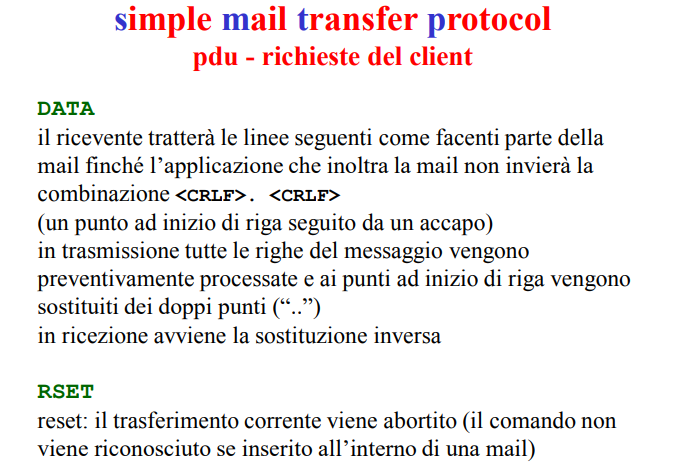
\includegraphics[width=10cm, height=6cm]{Screenshot 2025-01-06 135702.png} % Percorso dell'immagine
       % \caption{Arrivo in precedenza dei processi più piccoli} % Didascalia per la prima immagine
        \label{fig:sinistra} % Etichetta per riferimento
    \end{subfigure}
    \hspace{0.05\textwidth} % Spazio orizzontale tra le immagini
    % Immagine di destra
    \begin{subfigure}[t]{0.45\textwidth} % Sottotitolo di dimensione 45% della larghezza
        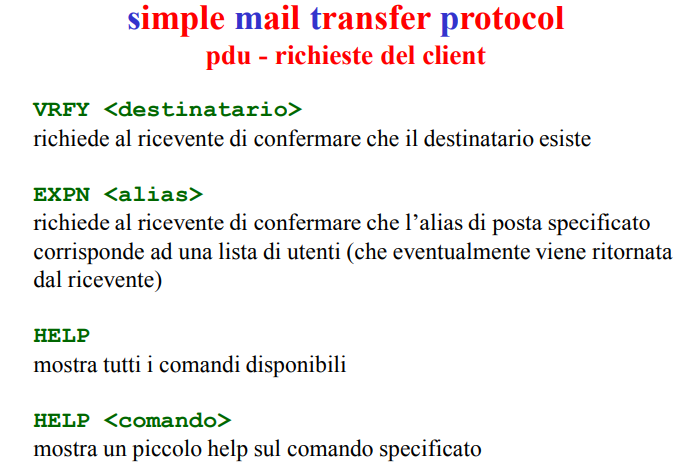
\includegraphics[width=10cm, height=6cm]{Screenshot 2025-01-06 135710.png} % Percorso dell'immagine
       % \caption{Arrivo in precedenza del processo più grande} % Didascalia per la seconda immagine
        \label{fig:destra} % Etichetta per riferimento
    \end{subfigure}
   % \caption{SJF/Shortest Job First} % Didascalia generale per la figura
    \label{fig:due_immagini} % Etichetta generale per riferimento
\end{figure}
\noindent
Per quanto riguarda le \textbf{risposte del server}: sono delle brevi frasi precedute da un codice numerico.
\subsubsection{Procedure e stati}
La transazione è iniziata dal comando \textbf{MAIL} che deve essere seguito dal comando \textbf{RCPT} e poi dal comando \textbf{DATA}. Il server entra in uno stato di accettazione del messaggio che termina nel momento in cui riceve la sequenza $<CRLF>.<CRLF>$ Nessun comando viene accettato durante il trasferimento del messaggio. La conversazione è terminata dal comando \textbf{QUIT}.
\subsection{POP3 (Post Office Protocol)}
I comandi del POP3 sono composti di quattro lettere, le risposte del server sono precedute da un \textbf{+OK} se positive o da un \textbf{-ERR} se negative.
\begin{figure}[H]
    \centering
    \begin{minipage}{0.55\textwidth} % Imposta la larghezza della colonna sinistra
        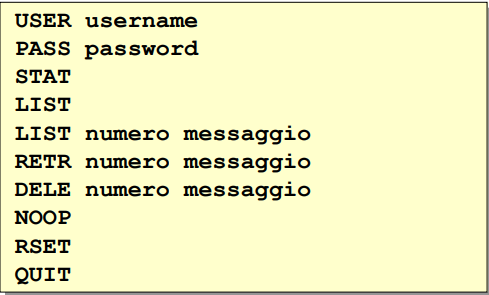
\includegraphics[width=9cm,height=4cm]{immagine_2025-01-06_140619499.png}
        %\caption{Routing by network address} % Opzionale
        \label{fig:immagine}
    \end{minipage}%
    \hfill
    \begin{minipage}{0.45\textwidth} % Imposta la larghezza della colonna destra
    Una sessione \textbf{pop3} attraversa vari stati: quando la connessione TCP è stata instaurata, pop3 entra nello stato \textbf{AUTHORIZATION} - in questo stato il client deve identificarsi. Quando ciò è avvenuto, il server acquisisce le risorse associate al client e la sessione entra nello stato \textbf{TRANSACTION} - in questo stato il client richiede servizi da parte del server. Quando il client spedisce il comando \textbf{QUIT}, la sessione entra nello stato \textbf{UPDATE} - in questo stato il server rilascia le risorse e la connessione TCP viene chiusa.
    \end{minipage}
\end{figure}
\noindent
\end{document}
 